
\section{Introduction}
A method can predict small perturbations poorly yet outperform local linearization on large finite interventions. For transcoders used in mechanistic interpretability, that possibility creates a practical question: \emph{when does poor local response fidelity coexist with useful prediction of a native downstream effect, and what properties of the prediction error support that regime?}

We study a public Gemma-3-270M transcoder at layer 15, with fixed donor edits propagated through the remaining native network. A historically selected pronoun-readout result motivated a new test on 256 disjoint name-pair blocks. The held-out result is a dose-dependent ranking crossover: native Taylor is better at dose .05, whereas the transcoder is better at a full donor patch, including comparison with a FIT-trained ridge map and on a predeclared transfer template. This is accuracy of a predicted readout effect, not improved natural answers or validation of a replacement circuit. Here native Taylor uses the native branch Jacobian to predict a vector change, which is then propagated through the exact nonlinear native suffix; it is neither the transcoder's Jacobian nor a first-order approximation of the final scalar readout.

A second public artifact, Gemma-3-1B layer 22, separates two claims that the first result alone could conflate. On 256 additional disjoint blocks, Taylor again wins at small dose and loses to the transcoder at larger doses. Yet at the full donor patch the transcoder is worse than zero change, ridge and the FIT class mean. Useful high accuracy therefore does not follow from beating Taylor. The full curve also matters: at dose 2 the transcoder beats zero change and the class mean, but still loses to ridge.

We investigate the first artifact's residual geometry using existing states rather than another fresh confirmation. A new 32-block experiment substitutes whole residuals from the same dose and condition with matched norms; a separate mask intervention tests FIT-selected switching groups. These controls avoid the dose-independent baseline mismatch of our earlier 16-block substitution study. They constrain the effect of specified residual directions and feature-mask changes, while unequal actual switching strength prevents interpreting the selected-versus-random contrast as isolated feature identity or a native circuit. The complete-cache diagnosis and earlier experiment remain separately reported secondary evidence. We now distinguish failed unscaled disjoint-group matching from a changed, equal-vector-norm estimand. A fresh lexical cohort tests the latter with fixed groups and scale; it descriptively reproduces a prediction-direction contrast on the same artifact, without a prespecified inferential decision or a complete explanation of crossover.

A separate Qwen3-0.6B component test provides a boundary: its measured CLT delta remains near the zero-change baseline across the dose curve. Gemma and Qwen differ in artifact, layer, suffix and readout, so their contrast cannot isolate a model-family cause. Historical failed forecasts and selected controls are retained in the appendices; they are not pooled with the fresh test or the posthoc mechanism sample as independent replications.
\subsection*{Relationship to the companion repair study}
The companion manuscript, \emph{When Oracle Low-Rank Error Repair Helps or Harms Intervention Predictions}, evaluates partial oracle repair and learned correction of vector predictions. Its separate layer-21 learned-correction study does not supply a new transcoder-dose result here. The present manuscript evaluates public-transcoder dose-response fidelity. The Qwen-0.6B analyses share captured native states and selected unit-dose outputs; they are not independent replications. Table~\ref{tab:shared} specifies the overlap. In particular, the adopted B ridge is the first fixed $P_{r1}$ trained on 128 FIT\_MAP examples, not the companion's pooled Direct256 predictor.
\begin{table}[ht]\centering\scriptsize
\setlength{\tabcolsep}{4pt}
\begin{tabular}{>{\raggedright\arraybackslash}p{.15\textwidth}>{\raggedright\arraybackslash}p{.38\textwidth}>{\raggedright\arraybackslash}p{.39\textwidth}}\toprule
Scope & Shared data or distinct acquisition & Unique measurement and estimand\\\midrule
Qwen-0.6B A/B & Same Base checkpoint, L27, is--are; 256 T2/T5 blocks, 2048 contexts, donor pairs and native $x,R,y$. B adopts $P_{r1}$ (FIT\_MAP128), 2048 native and 2048 $P_{r1}$ margins at $c=1$: 4096 outputs. & A: three fixed $P/U$ pairs, inside/outside oracle repair, forecasts, learned gate, full residual and Direct256. B: public CLT component, frozen mask, native Taylor and six-dose effect prediction. Other-dose ridge/mean use their own fixed dose-specific FIT labels.\\[3pt]
Gemma-270M A & Agreement T2/T5 corpus, 2048 contexts, L17, is--are; three accepted $P/U$ pairs. & Repair of intervention predictions at the last block; separate from the Gemma B native measurements.\\[3pt]
Gemma-270M B & Pronoun so/when/transfer corpus, 1536 contexts, L15, she--he; separate FIT and PILOT. & One public transcoder, full/projected dose response through dynamic native layers 16/17. Cache and residual follow-ups reuse B; they do not enlarge its independent sample.\\\bottomrule
\end{tabular}
\caption{Companion-study overlap. Common contexts and reused outputs are disclosed rather than counted twice as independent evidence. No public companion identifier has yet been assigned.}\label{tab:shared}
\end{table}

\section{Related work}
Transcoder-based circuits and their validation are established topics \citep{dunefsky2024,ameisen2025}. JumpReLU has an explicitly discontinuous threshold \citep{rajamanoharan2024}; threshold crossings are therefore not a newly discovered property. Computational sparsity is also the object of Jacobian sparse autoencoders \citep{farnik2025}, although sparsifying a Jacobian is different from matching a native MLP's Jacobian. Shabalin and Piotrowski directly examine transcoder-feature correspondence and Jacobian fidelity \citep{shabalin2026}.

JSAEs also compare Jacobians with finite latent interventions and discuss threshold-crossing exceptions; their SAE-decoder--MLP--SAE-encoder map differs from our native-versus-transcoder delta comparison \citep{farnik2025}. Ladner and Althoff study MLP--replacement discrepancy over continuous sets of internal activations using adversarial lower bounds and formal upper bounds \citep{ladner2026}. Our baseline-subtracted dose response and native-suffix readouts address a different estimand. These are already established neighboring questions, not newly discovered objections to this study.

Zhang et al. show that intervention-strength controls can change comparisons across sparse autoencoder codes \citep{zhang2026}. Their code-refit and output-calibration experiments differ from our fixed public-transcoder predictions of native MLP changes. The same coefficient $c$ need not give equal full- and projected-edit norms; our operator comparisons therefore describe the specified edits rather than an isolated causal effect of operator identity.

Zhang and Wang analyze failures of first-order attribution patching and propose a second-order correction for downstream nonlinearity \citep{zhangwang2026}. Our native Taylor comparator instead linearizes the branch's vector response and then applies the exact nonlinear native suffix. Its finite-dose error cannot therefore be attributed to replacing that suffix by a scalar first-order approximation; the approximated branch vector can still lead to a large readout error. The two baselines address related but distinct approximations.

Baz\'an S\'anchez tests whether a measured midpoint feature ablation predicts complete removal in transcoder replacement systems \citep{bazan2026}. That already provides a precedent for finite-dose prediction and frozen held-out forecasts. Its endpoint is a target feature's preactivation inside the replacement model; here the reference is a native branch change scored through the remaining native network. Our public TC prediction does not use a measured intermediate TEST intervention effect as its input. Neither comparison by itself establishes a complete causal mechanism.

Our central empirical contribution is a held-out dose-dependent reversal between public transcoders and native-vector Taylor, with an important separation between rank and accuracy. The selected 270M artifact also beats FIT-trained ridge at the full patch and transfers across templates; the 1B artifact repeats the crossover but does not repeat that accuracy advantage. Same-dose residual substitutions and restricted mask changes provide conditional diagnostics of the first artifact, not a training-cause identification. The negative Qwen component delimits the evidence further. We do not claim invention of Jacobian comparison, replacement-model validation, or attribution-versus-intervention testing. Novelty is bounded by the reviewed literature, not worldwide priority.

Lange et al. show that cross-layer transcoder objectives can favor shortcuts that omit intermediate computations \citep{lange2026}. This is relevant context for interpreting CLT-derived circuits, but our negative Qwen follow-up measures one local source-27--target-27 component. It neither evaluates the whole CLT graph nor establishes such shortcuts as the cause of that component's errors.

\section{What is predicted and how is it measured?}
Let $f(z)$ be the selected native branch, with its documented normalization, and $T(z)$ the fixed public transcoder. For recipient input $z$, donor difference $d=z_d-z$ and a unit FIT class-mean direction $w$, the tested edits are
\[
 \delta_{full}=cd,\qquad \delta_{proj}=c(d^\top w)w,
 \qquad c\in\{.05,.1,.25,.5,1,2\}.
\]
The same coefficient does not imply equal edit norms for the two operators. The target vector change and two principal predictions are
\[
 \Delta_N=f(z+\delta)-f(z),\qquad
 \Delta_T=T(z+\delta)-T(z),\qquad
 \Delta_J=J_f(z)\delta.
\]
Each predicted vector is added to the recipient's native branch output and propagated through the exact remaining native computation, including dynamic attention in Gemma layers 16 and 17. Native Taylor means the \emph{vector} branch JVP followed by this nonlinear suffix, not a scalar linearization of the entire readout.

Let $m_N$ be the native intervention's change in the she-minus-he logit margin, and $m_v$ the change predicted by vector $v$. We report pooled relative RMS error
\[
 \epsilon_v=\sqrt{\frac{\sum_i(m_{v,i}-m_{N,i})^2}{\sum_i m_{N,i}^2}}.
\]
Zero change has $\epsilon=1$. The denominator is uncentered signal energy; $1-\epsilon^2$ is not generally explained variance. Absolute RMS error and native signal RMS are reported alongside this ratio. All predictors share the denominator within a fixed cell, so their ranking within that cell is unchanged by normalization.

The selected Gemma transcoder has no affine skip, and the native model has no final-logit softcap. Neither is an available explanation to ablate. Frozen mask holds the baseline transcoder feature mask fixed. FIT class-cell means and ridge maps ($\lambda=.01$, global input RMS and centered intercept) predict native vector deltas without TEST labels. Their native FIT information and the public transcoder's pretraining costs are not matched. The intervention boundary is the output of post-feedforward normalization at layer 15, at the final token, rather than a raw down-projection or the residual stream. Technical prefix/suffix parity was qualified separately.
\section{Held-out Gemma test: a dose-dependent crossover}
\label{sec:newtest}

After the historical artifact/regime selection, a new campaign froze Gemma-3-270M, layer 15, the medium public transcoder, the six-dose grid and both input-edit operators before TEST. Its vector-only FIT used 32 name-pair blocks and 128 natural states across so/when; it fixed the class-mean projection direction, class-cell means and ridge baselines ($\lambda=.01$, global input RMS, centered intercept). A separate 32-block PILOT preceded TEST. TEST contains 256 disjoint name-pair blocks, two sides and three template forms, including a predeclared transfer form: 1536 recipient documents in total. The primary descriptive summaries below use the two original forms, 1024 documents. The selected artifact and task regime remain conditional choices, not a random sample of models or readouts.

A separately checked exact-prefix reuse path agreed with full native execution in its fixed technical qualification; no frozen-attention or final-layer shortcut is used. All predictors are scored through that same dynamic native suffix. MEAN and RIDGE use only the original FIT native-vector labels, never TEST deltas or readout targets; historical affine artifacts are separate comparisons.

\begin{table}[ht]
\centering\small
\begin{tabular}{lrrr}
\toprule Predictor & Full $c=1$ & Projected $c=1$ & Full $c=.05$\\
\midrule
Transcoder & \textbf{10.11} & \textbf{11.07} &117.46\\
Native Taylor &129.96&128.09&\textbf{12.10}\\
Frozen mask &108.35&108.06&110.16\\
FIT class-cell mean &57.73&57.94&127.72\\
FIT ridge &28.05&32.53&173.81\\
Zero change &100.00&100.00&100.00\\
\bottomrule
\end{tabular}
\caption{New TEST pooled relative RMS margin-prediction error, in percent. Each column contains 256 blocks, equally weighting the two sides and so/when templates within every block. Energies are pooled before taking a ratio or square root. These are descriptive finite-corpus summaries, not percentages of correct answers or population hypothesis decisions.}\label{tab:newtest}
\end{table}

The ranking reversal is also present in absolute error. On this same main-template mixture at $c=0.05$, TC and Taylor have RMS margin errors of 0.06030 and 0.00621 logits; at $c=1$, TC, Taylor and ridge have errors of 0.34963, 4.49225 and 0.96966 logits. The TC's absolute error therefore grows with dose, while the native signal grows faster (RMS 0.05134 to 3.45655 logits), reducing relative error. Within each fixed dose/operator/template cell, however, all methods share the same native-signal denominator: their ranking is not created by differing normalization denominators. This separates the measured method comparison from a causal explanation of why that comparison changes with dose.


The TC has substantially lower finite-readout error than zero, Taylor and the learned comparators at the large dose. This comparison is stronger than superiority to zero alone, but the ridge predictor receives native FIT labels unavailable to an uncalibrated public TC; public TC training cost is also not matched. At the small dose, TC is worse than zero and about 9.7 times Taylor in relative RMS. Thus the large-dose advantage does not establish local response fidelity.

For projected $c=1$, TC absolute RMS error is 0.34982 logits and native RMS change is 3.16014 logits. For the full operator at $c=1$, the error is 9.58\% on so and 11.01\% on when, compared with the historically selected 5.31\% and 6.32\%. The new TEST therefore reproduces a useful large-dose regime qualitatively, not the exact historical accuracy level. Its scale is compatible with the preceding new PILOT's 11.65\% and 11.92\% descriptive errors.

The original complete frozen TEST analysis reports: 288 descriptive cells (six methods, six doses, two operators, and three templates plus the main-template mixture), 36 endpoint-energy diagnostics, and five finite-cohort contrasts. All 18432 result records were independently aggregated for those original outputs. The later residual-geometry cache analysis below is a separate posthoc analysis, not additional acquisition. Figure~\ref{fig:newdose} presents the new TEST as the central dose comparison; method-specific markers and line styles identify curves independently of color; Appendix~\ref{app:fullgrid} retains every dose and method.

\begin{figure}[ht]
\centering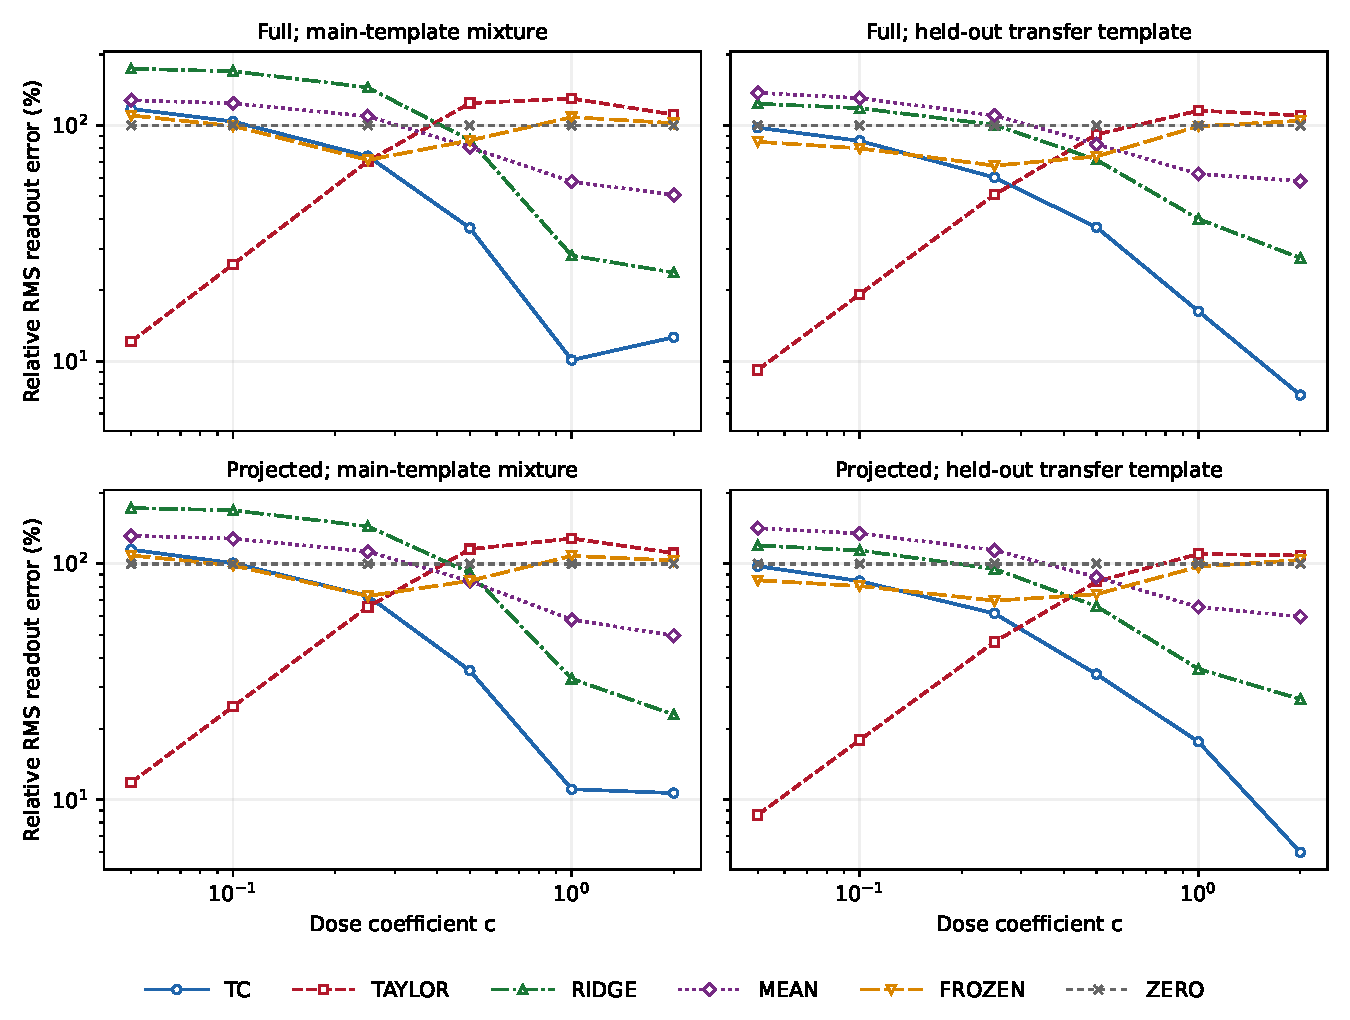
\includegraphics[width=\linewidth]{figures/new_test_dose.pdf}
\caption{Complete new 256-block TEST dose curves. Main-template mixture and transfer are displayed separately. Points are descriptive pooled relative RMS errors; connecting lines guide the eye and do not establish behavior between measured doses.}\label{fig:newdose}
\end{figure}

On the predeclared third transfer template at full dose, TC relative RMS error is 16.28\% for the full operator and 17.59\% for the projected operator. Full-operator Taylor and ridge errors are 115.44\% and 40.10\%; projected errors are 110.05\% and 35.83\%. Thus the large-dose advantage transfers to this template, with weaker accuracy than the original-template mixture. At dose .05, transfer TC error is 97.78\%/97.73\% for full/projected edits. No qualified interval is assigned to transfer or these small-dose cells.

The predefined 12 joint TC intervals at $c=1$ are now computed. For the main-template mixture, full-operator relative RMS is 10.11\%, with interval [8.99\%,11.38\%]; projected is 11.07\%, with interval [9.78\%,12.53\%]. These paired studentized log-RMS intervals have a construction confidence of 99\% and finite-scenario qualification; they are not a distribution-free guarantee. The desired simultaneous width target was not met: projected/when relative RMS has halfwidth 2.431 percentage points, exceeding the 2-point target. The other eleven metric widths meet their targets. Qualification of the interval method and attainment of an actual width target are separate outcomes. The complete interval table is in the evidence bundle.

The input direction and learned baselines were frozen before the respective PILOT/TEST access. None was selected by the signs in Table~\ref{tab:newtest}. Operation counts and review boundaries are retained in Appendix~\ref{app:costs}.


\section{A second artifact: crossover without the same accuracy}\label{sec:second}
We selected the locally available public Gemma-3-1B layer-22 medium 16k, $L_0=60$, no-affine transcoder by an availability/depth rule, before acquiring these outcomes. This artifact had historical exploratory exposure (Appendix historical outcomes); artifact selection is not blind. The new protocol froze 32 fresh FIT name-pair blocks and 256 fresh TEST blocks, disjoint from the earlier observed lexical pools. This is experimental-cohort separation, not a claim about pretraining exposure. The so, when and transfer frames share TEST names; transfer is a template test, not another independent lexical sample.

The full donor operator uses all six doses and the same six comparator classes. Native Taylor is a vector JVP, followed by the exact nonlinear native suffix (layers 23--25 and final normalization/head), as are the other predictions. The readout is she minus he. Ridge uses the fixed FIT protocol ($\lambda=.01$); the main mixture pools so/when. Table~\ref{tab:secondkey} highlights the distinction between rank and accuracy. Figure~\ref{fig:second} and Appendix~\ref{app:secondcurve} retain the entire curve, including unfavorable cells. All 144 method/frame/dose metrics are supplied; 9216 rows are dependent measurements of 256 blocks, not 9216 independent samples.
\begin{table}[ht]\centering\small
\begin{tabular}{lrrrrr}\toprule
Condition & TC & Taylor & Ridge & Mean & Zero\\\midrule
Main, $c=.05$ &134.18&23.56&84.78&94.91&100\\
Main, $c=1$ &115.38&269.86&50.80&66.99&100\\
Main, $c=2$ &41.86&110.86&34.63&43.73&100\\
Transfer, $c=1$ &137.43&267.26&60.81&---&100\\\bottomrule
\end{tabular}
\caption{Second artifact: relative RMS error (percent). The dash omits a value only from this compact display; all methods and doses are in Appendix~\ref{app:secondcurve}.}\label{tab:secondkey}
\end{table}
\begin{figure}[ht]\centering
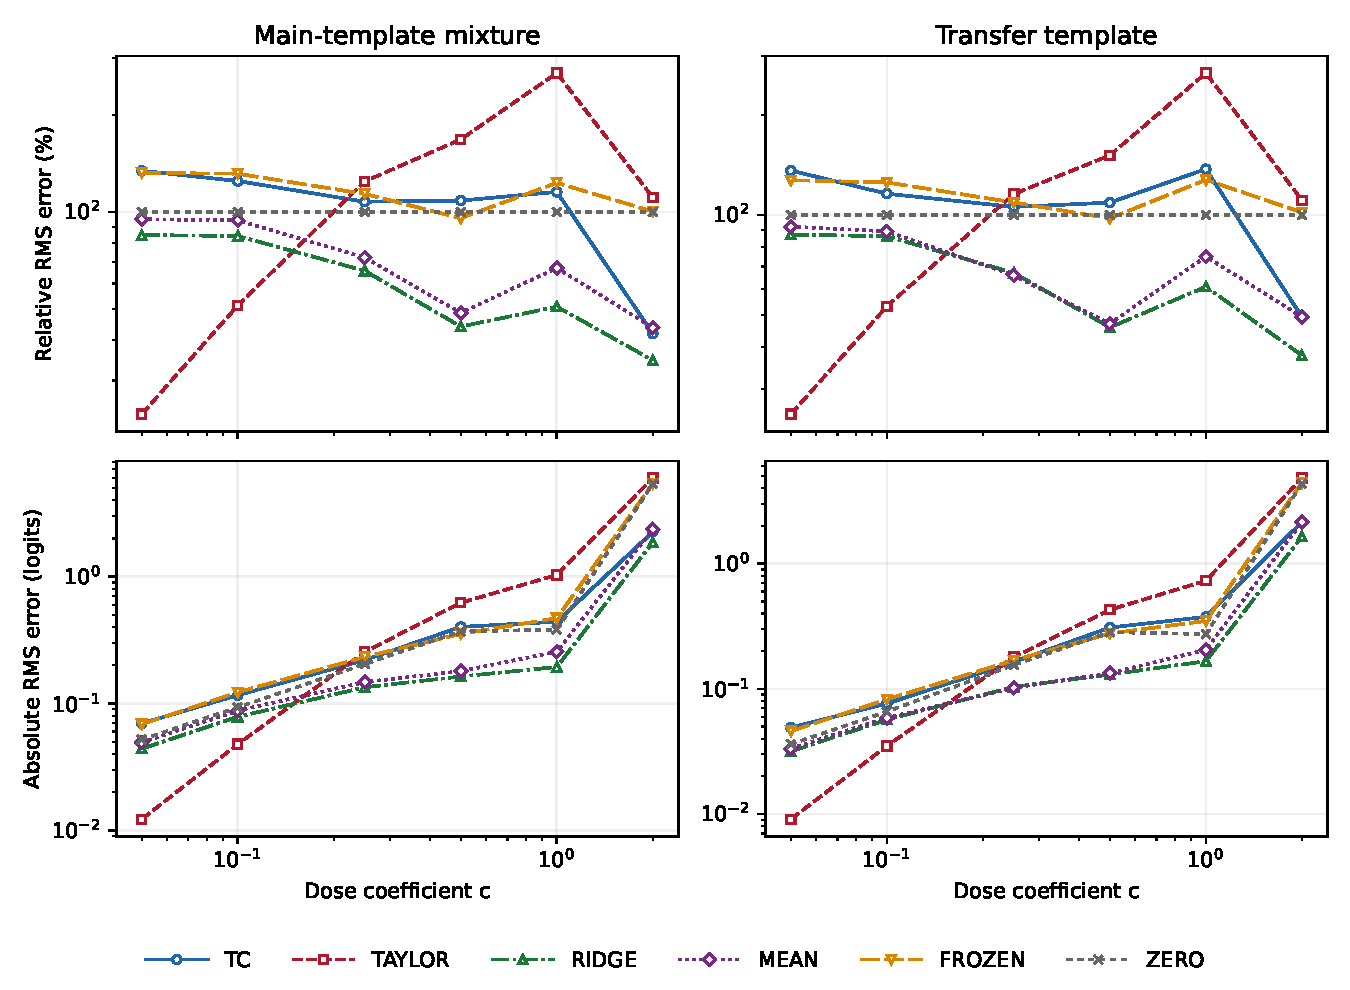
\includegraphics[width=\textwidth]{figures/second_artifact_dose.pdf}
\caption{The second artifact repeats the TC--Taylor crossover but not the first artifact's high full-patch accuracy. Relative and absolute RMS rankings agree within each condition. At dose 2 the TC beats zero change and the class mean on the main mixture, but ridge remains better. Templates share lexical blocks.}\label{fig:second}
\end{figure}
At $c=1$, TC absolute RMS is .4406 logits versus Taylor's 1.0306 and ridge's .1940; native RMS is .3819. Its nominal pointwise 95\% block-bootstrap interval for relative RMS is [112.72\%,118.25\%], conditional on the fixed FIT objects. These intervals use 1999 frozen-seed resamples and do not inherit the earlier 270M qualification or establish familywise population decisions. Transfer TC error also exceeds frozen-mask error (127.55\%). The result is a replication of ranking reversal, not a second demonstration of approximately 10\% error or superiority over learned predictors.

\section{Same-dose residual and selected-switch diagnostics}\label{sec:samedose}
Two posthoc tests reuse 32 previously observed 270M blocks (indices 16--47), distinct from the earlier 16-block sample. Three frames, two directions, two operators and doses .05/1 yield 768 conditions. These are controlled interventions on predictions with fixed native targets, not fresh held-out mechanism confirmation.
\subsection{Whole residuals at matched dose and norm}
For native target change $n_i$ and TC prediction $t_i$, define $r_i=t_i-n_i$. We replace the prediction by $n_i+\|r_i\|r_j/\|r_j\|$, with two prespecified cyclic partner shifts (1 and 7) within the same frame, direction, operator and dose. This uses oracle native targets. It replaces the \emph{whole} residual, rather than replacing an endpoint baseline error, and adds no dose-independent baseline mismatch. Norm matching is checked after FP32 rounding; the resulting prediction is scored through the exact native suffix.

For full edits at $c=1$, pooled mean squared readout error is .11153 for the original residual, versus .14940 and .18659 for the two substitutions. For projected edits it is .12119 versus .23641 and .25200. Each full-dose frame favors the original direction against both partners. This is conditional evidence for favorable residual orientation under these constructions. It is not universal: transfer/full at $c=.05$ improves under partner 7 (mean loss difference $-.0001594$). Appendix~\ref{app:samedose} retains every stratum. Different partners, samples and constructions mean that this result does not overwrite the earlier 16-block operator reversal.
\subsection{Restricting feature-mask changes}
Let $a_0,a_1$ be preactivations, $m_0,m_1$ the corresponding JumpReLU threshold masks, and $u_1=\operatorname{ReLU}(a_1)$. Define $h_{base}=u_1m_0$ and $s=u_1(m_1-m_0)$. For a group $G$, ONLY uses $h_{base}+1_Gs$ and EXCEPT uses $h_{base}+(1-1_G)s$. Each code is decoded with the original decoder/bias, baseline-subtracted and scored through the native suffix. Endpoint magnitudes and nonswitching features remain; ONLY does \emph{not} mean a 32-feature circuit. BASE can differ from the archived frozen-mask linear predictor because of endpoint ReLU clamping.

The group contains the top 32 FIT-scored features by mean absolute switch contribution times decoder-row norm; a fixed-seed random group of 32 is drawn from its complement. No TEST outcomes select either group. At full dose/full edits, ONLY-top yields .10463 MSE versus the original .11153, whereas EXCEPT-top yields 8.93294. Thus the selected group's mask changes approximately preserve prediction accuracy under this intervention, and removing them is highly damaging. Projected full-dose values are .11782 and 7.45841 versus .12119 originally. At small dose removing the group instead slightly improves pooled loss; we do not promote only the favorable conditions.

The random comparison is \emph{not strength matched}. At full dose/full edits, the selected group switches an average 8.3125 features versus .02083 for random; random has zero switches in 188/192 contexts. Projected full-dose random is inactive in 191/192 contexts. Equal group cardinality therefore does not isolate feature identity at equal actual switch count or intervention norm. These bounded posthoc diagnostics establish conditional importance of specified mask changes in the replacement prediction, not faithful native features, a native circuit, or an additive percentage explanation of the crossover.


\subsection{Failed strength matching and equal-norm prediction directions}\label{sec:normnew}
A cache-only follow-up used the actual 32 FIT blocks and 128 recipient documents (64 each in \emph{so}/\emph{when}), correcting an earlier report's scope label. All five fixed size-32 alternative groups, each disjoint from top32, failed joint count/norm matching: their mean counts were 6.05--6.19 versus 10.375 for top32, and norms 211.47--222.38 versus 747.39. A post-run triangle-inequality certificate bounds the mean norm of \emph{any} size-32 group disjoint from top32 by 441.559, implying a norm-distribution Wasserstein-1 distance of at least 305.828, above the fixed descriptive FIT band 207.058. This is a pooled finite-FIT support bound, not a framewise impossibility proof or equivalence test. The five overlapping alternatives share 28--31 features with one another; they remain failed unscaled strength controls.

A separately reviewed follow-up changed the estimand. Write $S_G$ for the summed signed threshold-switch decoder contribution of group $G$, and construct
\[
 y_G=y_{\mathrm{TC\_FULL}}-\rho S_G/\|S_G\|,\qquad \rho=101.51097375005.
\]
The six groups and pooled FIT scale were fixed before the new readouts; native error was not used to construct the directions. Joint eligibility requires all six norms to permit amplification at most four. These are norm-rescaled EXCEPT-minus-FULL prediction directions around TC\_FULL/RR, scored through the native suffix, not equalized native switch counts, native feature ablations or a native circuit. The historical ON arm refers to positive crossings, not TC\_FULL. Endpoint magnitudes and nonswitching contributions remain. The primary statistic is the equal-block top32 MSE increment relative to TC\_FULL minus the equal mean of five alternative-group increments. A positive value means removing the top direction damages prediction more than removing the control directions.

\begin{table}[ht]
\centering\small
\begin{tabular}{lrrr}\toprule
Cohort/frame & Eligible contexts & Blocks & Top minus controls\\\midrule
Exposed historical so/when &128/128&32/32& .165807\\
Fresh lexical so/when &128/128&32/32& .198352\\
Fresh changed-context transfer &45/64&26/32& .083652\\
Fresh object construction/readout &12/64&9/32& .013883\\\bottomrule
\end{tabular}
\caption{Equal-norm direction diagnostic, full donor edit at dose 1; MSE-increment units. Positive contrasts measure relative prediction damage. Coverage is conditional on joint six-direction eligibility.}\label{tab:normnew}
\end{table}
The historical result is posthoc on already exposed outcomes. The fresh experiment fixes the same groups and scale on 32 new, disjoint exclusive-name-category pairs (256 contexts total), without readout-based refitting or selection. Its primary \emph{so}/\emph{when} descriptive replication concerns the same Gemma-270M/L15 artifact and she-minus-he readout. Changed-context transfer retains that readout; the object frame changes both construction (``receptionist greeted'') and readout to her-minus-him, so token identity is not isolated. Its 12/64-context, nine-block eligibility is a severe limitation: the positive eligible-subset result cannot establish broad object-readout transfer. Controls overlap and are not five independent replications. A cache reconstruction finds one to four unique control directions per eligible context; top32 is distinct in every eligible case. Identical entries reflect identical active switch coefficients and FP32 targets, rather than copied outcomes. The frozen equal mean weights each unique direction by its multiplicity divided by five. Inference units are lexical blocks, not groups or aliased suffix calls; no posthoc deduplication changes that estimand. Full counts are in Appendix~\ref{app:normnew}. No new-model generalization or complete crossover mechanism follows. All three stages have genuine independent completion approvals; preserved reports' pending lines are superseded by those receipts.

For a signed native readout margin $m_N$, let $e=m_{\mathrm{TC\_FULL}}-m_N$ and $\Delta m=m_G-m_{\mathrm{TC\_FULL}}$. The exact loss increment is
\[
 (e+\Delta m)^2-e^2=(\Delta m)^2+2e\Delta m.
\]
Thus a large readout sensitivity need not worsen prediction: its alignment with the existing signed error also matters. Approximate collinearity of top32's direction with the predicted TC delta is an untested explanatory hypothesis here, not an observed mechanism. A gradient at TC\_FULL has not been measured in these follow-ups; earlier gradients at the natural or native endpoint do not supply it. A future direction/gradient test would require its own protocol and accounting.

\section{Earlier diagnostics and their limits}\label{sec:mechanism}
The complete 270M cache and an earlier posthoc oracle experiment on the first 16 observed blocks supply secondary evidence (Appendix~\ref{app:earlierdiagnostics}). They are distinct from the new 32-block tests and do not add independent replications. Complete-cache endpoint alignment depends on whether centering occurs within or across frames; pooled cancellation is therefore not a sufficient explanation of readout accuracy.

The earlier experiment replaced a baseline endpoint error before crossing residual norm and direction. Its replacement satisfies $r_P(c)=r(c)+e_{0,i}-e_{0,\mathrm{partner}}$: a mismatch that need not vanish at small dose. Consequently, small-dose norm inflation is partly built into the construction. At full dose, the norm-matched direction contrast favored the original residual for full edits but not projected edits. The newer whole-residual substitution has different partners and blocks and adds no such baseline mismatch; its different projected-edit outcome is not a contradictory repeat of the same test.

Earlier gradient-parallel/perpendicular interventions used unequal norms, and the magnitude--direction experiment showed large interactions. Neither supports additive mechanism percentages. All constructions use native truth and remain bounded posthoc oracle diagnostics; full definitions, outcomes and negative strata are preserved in the appendix.
\section{A negative boundary: the Qwen0.6 component}
\label{sec:qwen}

A separately frozen extension evaluates the public Qwen3-0.6B-Base source-27--target-27 CLT component, not the whole CLT graph or historical E041's layer 21. Full donor edits use the same six doses, with predictions scored through the final native normalization/head for the is-minus-are readout. The 256 lexical blocks and two frames are shared with companion analyses; already exposed unit-dose native/ridge outputs are reused. Other-dose FIT comparators were fixed before new B outcomes. This is a descriptive shared-cohort boundary, not independent fresh confirmation. Native Taylor predicts the branch vector before exact downstream scoring; composed scalar linearization is a separate comparator. Implementation and adoption details are in Appendix~\ref{app:qwenimplementation}.

\begin{table}[ht]
\centering\small
\begin{tabular}{lrr}
\toprule Predictor & Qwen mixture $c=.05$ & Qwen mixture $c=1$\\\midrule
CLT component &99.830&100.347\\
Native vector Taylor &3.172&34.600\\
Composed scalar linear &3.305&35.904\\
Frozen recipient mask &99.830&100.302\\
FIT ridge &36.499&30.572\\
FIT conditional mean &37.589&37.757\\
Zero change &100.000&100.000\\\bottomrule
\end{tabular}
\caption{Qwen0.6 follow-up: pooled relative RMS readout error in percent. The two frame distributions and all six doses are retained in Appendix~\ref{app:qwen}; this is a shared-cohort descriptive extension, not a fresh independent confirmation of the Gemma effect.}\label{tab:qwen}
\end{table}

The CLT component's relative RMS error stays close to the 100\% zero-change baseline across the tested curve; no Gemma-like positive regime appears. At $c=1$, its absolute RMS error is 2.45515 logits, versus 0.84654 for Taylor and 0.74800 for ridge, with native signal RMS 2.44665. The two frames separately give CLT errors 100.022\% and 100.625\%. These findings constrain generalization of the selected Gemma success; they do not isolate model size, architecture, training, readout or suffix depth, which all differ. Nor do they establish that the entire CLT graph is unfaithful or identify a hook-scale defect. The declared normalized-MLP-input operator and four technical branch/head/JVP/reachability checks were independently accepted; those controls are not a global fidelity certificate.

\section{Discussion and conclusion}
The strongest positive result remains the 270M held-out full-patch prediction and predeclared template transfer. The second artifact changes the generalization claim: the Taylor--TC ranking crossover repeats, but useful full-patch accuracy does not. At $c=1$ its TC loses to zero change, ridge and mean despite beating Taylor; at $c=2$ it beats zero and mean but not ridge. Reporting the full curve avoids conflating these outcomes. All methods within a condition have the same relative-error denominator; the ranking reversal also occurs in absolute error. Neither artifact establishes decreasing absolute TC error with dose or general replacement-model faithfulness.

The bounded posthoc oracle diagnostics using same-dose, norm-matched whole-residual substitutions show favorable original orientation in every full-dose frame against two partners, with a small-dose exception retained. The selected-switch test shows that a FIT-selected group's mask changes preserve much of the first artifact's full-patch accuracy under the specified replacement operation. Its nearly inactive random control cannot isolate identity at equal strength, and the experiment preserves endpoint magnitudes and other features. It therefore provides a bounded intervention diagnosis, not a recovered native circuit. The new norm-rescaled direction test addresses one strength confound by changing the intervention, and fresh lexical data descriptively reproduce its positive prediction-damage contrast. No formal significance, confidence-interval or prespecified decision claim is attached to this follow-up. Failed unscaled matching remains a distinct negative result. The restricted transfer and especially object eligibility constrain generalization; equal output norm still does not equalize switch count, semantic content or curvature. The earlier 16-block baseline-error substitution is a different construction with a dose-independent mismatch and substantial interactions; its operator-dependent findings remain secondary rather than being combined into an additive mechanism account.

Scope and inference remain explicit. Both public Gemma artifacts had historical exposure; their new lexical tests use fixed acquisition protocols. The 32- and 16-block diagnostics reuse observed data. The Qwen component remains a negative boundary, not an architecture-controlled comparison. Synthetic contexts, selected branches and two-token readouts do not measure general answer quality. The original hypothesis family failed calibration; separately qualified 270M intervals cover only their own metrics, while the second-artifact intervals are nominal pointwise estimates conditional on FIT. Shared templates and repeated measurements do not enlarge the number of independent blocks. Historical failures and all new unfavorable conditions are retained.

Local fidelity, ranking against a local approximation, useful finite-effect accuracy and a mechanistic explanation are separate empirical claims. The evidence supports the first artifact's conditional usefulness and a repeated ranking crossover, while limiting both generalization and the interpretation of its switching and residual geometry.
\clearpage
\appendix
\section{Historical designs and prespecified questions}
\subsection{Artifacts, tasks, and dependence}
The extended study uses Gemma-3-270M (layers 5, 9, 15), Gemma-3-1B (7, 13, 22), and GPT-2 (ReLU artifacts at layers 6/9 and a TopK artifact at layer 9). Gemma Scope 2 JumpReLU artifacts have width 16k and small/medium/big activity labels; medium supplies the principal readout. The 18 Gemma artifacts are shared-model, shared-layer observations, not 18 independent populations. Earlier family measurements with invalid or conditional hooks are not silently counted as valid replications.

The local corpus contains 640 synthetic texts spanning agreement and pronoun tasks. The readout TEST uses six templates: four agreement constructions and two pronoun continuations, with 40 texts and 20 blocks per template/cell, or 240 texts per model--layer. Agreement readouts retain the conflicting head/distractor conditions specified in the pre-TEST cost amendment; local calculations retain all conditions. The two pronoun templates reuse name-pair blocks.

The patch grid is $c\in\{0.05,0.1,0.25,0.5,1,2\}$. Local norm-based doses use three fitting values $\{1/128,1/64,1/32\}$ and five test values $\{1/512,1/256,1/16,1/8,1/4\}$. Local and donor-patch dose units are different and should not be put on a single numerical axis without conversion.

\subsection{The H1--H4 questions}
\textbf{H1: large finite readout mismatch.} At full patch $c=1$, require a median block error at least $5\times$ native Taylor and at least $0.3$. The original Gemma TC family has 36 cells; GPT-2 has 18, with separate frozen-mask families. The archived procedure resamples blocks 2000 times, counts failure of the conjunction, and applies Holm. We reproduce its decisions without claiming independently calibrated nominal coverage.

\textbf{H2: useful jump prediction.} Fit $R_J(t)=\kappa/t$ and test whether it beats all required baselines: nearest fitting dose, an anchored family-exponent model, and a free-exponent power model. Scores use median absolute log error over test blocks/doses, with a fixed nonzero-resolution rule. A constant baseline is reported but is not the sole criterion.

\textbf{H3: artifact-level scale prediction.} A threshold-density formula uses weights and natural/fitting activations to predict $\kappa$, with a frozen-transcoder-response denominator rather than access to the native test response. Its primary criterion requires SVA Spearman correlation at least $0.7$ and greater than the absolute correlations of L0 and threshold-mass baselines over 18 Gemma artifacts. This tests an aggregate ranking, not individual-intervention selection.

\textbf{H4: attribution versus native input edit.} Require median attribution--native correlation below $0.8$ and a paired improvement of at least $0.1$ for TC-edit, with the recorded CI above zero. The bootstrap $p$ tests positivity, not whether the true improvement exceeds $0.1$. We retain that distinction.

\section{Historical outcomes and selected controls}

\subsection{Poor small-dose response survives good reconstruction}
An exploratory width/activity sweep on Gemma-3-1B contains 18 artifacts sharing 64 evaluation texts. At $t=1/128$, vector relative RMS is 1.225--2.942, versus native Taylor 0.01049--0.01663. At $1/8$, the transcoder range is 0.8536--1.1143. Better than a small-dose error of two does not make an error near one highly faithful.

Across six matched layer/activity-label comparisons, increasing width from 16k to 262k improves reconstruction in all six but worsens small-dose response in five. Actual activity and training are not matched, so this does not identify a causal effect of width. Mask-change associations likewise do not assign a causal share of error to jumps. The extended local study replicates the qualitative local mismatch across the two Gemma sizes, while GPT-2 shows a different jump profile; families remain confounded with model and training.

\subsection{The stronger full-patch mismatch hypothesis fails}
At $c=1$, H1 holds pointwise in 7/36 Gemma TC cells but in 0/36 after the recorded Holm procedure. Frozen mask holds pointwise in 5/36 and in 0/36 after correction. GPT-2 TC holds pointwise in 1/18, also with none after correction. The medians across Gemma's cell-wise block-median errors are 0.739 for TC and 0.511 for Taylor.

This is a failure of the stated strong forecast, not a demonstration of equivalence to the native model. Taylor itself is inaccurate at finite doses; requiring a fivefold excess is stringent when the baseline is already poor. Pointwise Gemma H1 successes occur at early layers with small native signals. Secondary projection results must be separated: a post hoc Holm calculation yields six Gemma TC rejections, also restricted to early layers. They do not reverse the primary full-patch decision.

\begin{table}[ht]
\centering\small
\begin{tabular}{p{.19\linewidth}p{.31\linewidth}p{.39\linewidth}}
\toprule Question & Fixed-test outcome & Interpretation boundary\\
\midrule
H1 & 0/36 Gemma full-patch TC after Holm & Does not establish faithfulness; finite Taylor is a weak reference.\\
H2 & 0/36 primary Gemma cells & Failure against required predictive baselines, not just an arbitrary scalar cutoff.\\
H3 & SVA task $\rho=0.860$; pronoun task $0.668$ & Pooled artifact association; no within-layer advantage over L0.\\
H4 & 4/12 Gemma cells, all in 270M & Input edits can alter multiple features; weaker positive effects also occur in 1B.\\
\bottomrule
\end{tabular}
\caption{Extended-study outcomes. These are distinct families/questions; their cells cannot be pooled as independent successes.}
\end{table}

\subsection{Dose models: predicting the sum is easier than the jump}
In the separate dose-law study, a fitting-based $F^2+\kappa/t$ model hits total squared relative error in 177/216 JumpReLU configuration--direction--dose cells, but jump energy in only 99/216. A hit is a multiplicative band $[0.8,1.25]$ on the \emph{squared} error. Cells reuse contexts; some historical doses/configurations were exposed. The weak recorded falsifier is not triggered, yet a continuous valid prefix from the smallest dose exists only in four of eight principal groups. This is not a universal dose law.

The extended H2 test is stricter in a different way: it compares prediction with required baselines on test blocks/doses. It succeeds in 0/36 primary cells; even pointwise M1 beats all three baselines in only 4/36. Its median absolute log score is 0.768 versus 0.529 for the nearest-dose baseline. Relaxing H1/H4 labels would not repair this comparison.

H3 supplies a bounded positive result: primary SVA correlation is 0.860, above the specified L0/mass correlations of absolute 0.635/0.695. Post hoc calibration gives $10^{\operatorname{median}|\log_{10}(\kappa_{pred}/\kappa_{obs})|}=1.30$ across 18 points. This avoids mistaking cancellation in a signed log median for calibration. Within each three-artifact layer group, L0 ranks just as well. Pronoun/task correlation 0.668 does not meet 0.7 despite positive baseline gaps.

The secondary random-direction H3 has an additional implementation mismatch: prediction averages 16 directions for all artifacts, but small/big measurement uses four; prediction averages ratios while observation pools energies. Its numerical impact has not been recomputed. We do not present random H3 as an aligned confirmation. The primary task-direction result is unaffected by that direction-count issue.

\subsection{A narrow strong success at a large dose}
After examining the matrix, we selected Gemma-270M/L15/medium on two pronoun templates for raw replay. The 80 saved NPZ records confirm large native effects and small readout prediction error (Table~\ref{tab:positive}). These are 40 texts/template and 20 shared blocks, not two independent population studies. The finite full-patch vector error is still 0.434/0.496, so the readout success does not imply accurate whole vectors.

\begin{table}[ht]
\centering\small
\begin{tabular}{llrrrr}
\toprule Template & Operator & $\epsilon_{TC}$ & Mean $|m_N|$ & $\epsilon_{F}$ & $\epsilon_{\mathrm{Tay}}$\\
\midrule
so & full &0.0531&5.384&1.128&1.482\\
when & full &0.0632&3.836&1.130&1.558\\
so & projected &0.0505&5.085&--&--\\
when & projected &0.0839&3.814&--&--\\
\bottomrule
\end{tabular}
\caption{Post hoc positive regime, $c=1$. Signal is in logits. $F$ is frozen mask, Tay is native Taylor; dashes leave secondary values to the accompanying JSON. TC sign agreement is 40/40 per cell. These are selected descriptive cells, not representative frequencies.}\label{tab:positive}
\end{table}

At full $c=1$, TC absolute RMS error is 0.292/0.256 logits, with correct signs on all 80 texts; frozen and Taylor have the opposite sign on all 80. At $c=0.05$, TC relative error is 2.64/3.15, but native mean absolute signals are only 0.034/0.022 logits. Absolute TC error is then smaller, 0.105/0.090. Relative and absolute errors describe different aspects of this reversal (Figure~\ref{fig:dose}).
\begin{figure}[ht]
\centering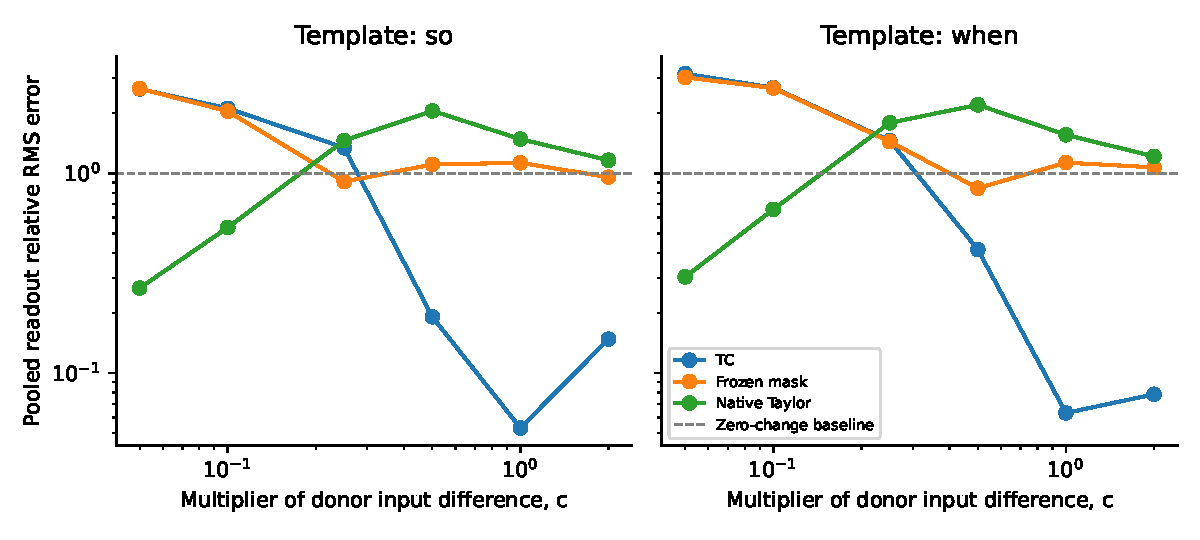
\includegraphics[width=\linewidth]{figures/dose.pdf}
\caption{Same post hoc selected artifact and texts under full-patch dose variation. Pooled readout error, not block-median H1. Small dose does not imply small relative prediction error; native Taylor also becomes inaccurate at large doses.}\label{fig:dose}
\end{figure}

Two additional controls narrow explanations. First, the projected patch is not simply the full donor endpoint: documented unit-direction projection and saved norms imply median omitted components of 42.7\%/53.2\% of the full input-difference norm. This is a conditional geometric inference, not a new vector replay or distance from the entire activation manifold.

Second, full-patch linear readout errors between $g^\top\Delta_T$ and $g^\top\Delta_N$ are 4.65\%/5.37\%; projected-patch errors are 4.67\%/6.85\%. Thus later nonlinear compression alone cannot explain the agreement. However, $g^\top\Delta_T$ versus the \emph{actual finite} native change has errors around 10.7--13.2\%; the two comparisons must not be conflated.

Signal size alone is not an established causal explanation either. One post hoc random-direction illustration has larger mean native changes, 8.536/7.104 logits, but worse relative errors 19.35\%/14.93\% and larger absolute errors. All 16 controls are retained in the supplementary data. This illustration is not a signal-matched experiment, and does not isolate dose from direction.



Earlier decoder-ablation comparisons gave nearly perfect attribution correlations, but tested linearity of the native suffix for those decoder directions. H4's native input edit is a stronger and different operation. Attribution--native rank correlation lies below 0.8 in all 12 Gemma cells; the full improvement criterion holds in 4/12, all 270M. In 1B, three smaller paired gains (0.093, 0.026, 0.077) have recorded Holm-adjusted positivity $p<0.05$, despite none meeting the full H4 criterion. This is a limited positive result, not permission to lower the original threshold. Spearman agreement does not guarantee accurate effect magnitudes, and TC-edit may benefit by capturing collateral feature changes.

\subsection{Earlier operator comparisons and a recovered dose-control record}
Two historical datasets clarify why the operator and the validity of the reference must be stated explicitly. They are descriptive supporting records with incomplete experiment-level review, rather than additional primary confirmations of H1--H4.

TC\_DOWNSTREAM uses 32 texts in eight blocks, two signs, and native downstream propagation in Gemma-3-1B. At dose $1/128$, medium-TC readout relative RMS errors are approximately 0.81 and 1.74 at L13 and L22, versus native Taylor 0.016 and 0.025. Meanwhile individual decoder-feature ablations have attribution correlations near 0.998--1.000. The latter change the decoder output linearly and chiefly test the native suffix on those directions; they do not validate prediction of an input edit to the native MLP. At dose $1/2$, L22 affine-TC error is about 0.33 versus Taylor 1.21. The affine and medium artifacts are distinct and cannot be spliced into one artifact's dose curve. The historical report has no dedicated complete independent raw-data acceptance, and tiny FP32 KL values are not used here as precise evidence.

The distinct, non-transcoder PORT\_P5 dose-control record is retained in Appendix~\ref{app:port}, rather than counted as additional evidence for TC faithfulness.


\section{Additional definitions for historical comparisons}

\subsection{Local vector responses}
Let $f(z)$ denote the native selected branch at its documented input coordinate, including a branch-specific normalization when applicable, and let $T(z)$ be the transcoder. For a perturbation $\delta$, define
\begin{equation}
 \Delta_N=f(z+\delta)-f(z),\quad
 \Delta_T=T(z+\delta)-T(z),\quad
 \Delta_J=J_f(z)\delta.
\end{equation}
The frozen-mask response $S$ holds the transcoder's baseline activation mask fixed; it includes a skip path when present. Let $J_{\mathrm{switch}}$ be the explicitly evaluated change due to switching the activation mask, as stored by the implementation. Set $A=S-\Delta_N$ and $E=\Delta_T-S-J_{\mathrm{switch}}$. Thus $E$ captures the recorded numerical remainder rather than adding a third term to an already exact two-term definition. Then
\begin{equation}
 \|\Delta_T-\Delta_N\|^2=\|A\|^2+\|J_{\mathrm{switch}}\|^2+\|E\|^2
 +2\langle A,J_{\mathrm{switch}}\rangle+2\langle A,E\rangle+2\langle J_{\mathrm{switch}},E\rangle.
\end{equation}
Cross terms can be negative and are stored once. A large jump norm is not an additive causal percentage of total error. We report pooled relative RMS $\sqrt{\sum\|\Delta_T-\Delta_N\|^2/\sum\|\Delta_N\|^2}$, cosine and norm diagnostics, and frozen/jump terms separately.

\subsection{Doses and operators}
One perturbation family uses $\delta=t\rho w$, where $w$ is a unit task direction and $\rho$ is a mean fitting-state norm. Another uses the input difference $d=z_{\mathrm{donor}}-z_{\mathrm{recipient}}$:
\begin{equation}
 \delta_{\mathrm{full}}=cd,\qquad
 \delta_{\mathrm{proj}}=c(d^\top w)w.
\end{equation}
The direction $w$ is estimated from fitting-class means. Random controls are covariance-matched combinations of fitting differences, normalized to the full-patch norm, not isotropic perturbations. A residual-stream perturbation is an additional operator, not automatically the same path at intermediate doses. Full and residual $c=1$ share a donor endpoint and are not counted as independent replications.

\subsection{Native suffix and readout}
Starting with the recipient's native branch output, insert $\Delta_N$, $\Delta_T$, $S$, or $\Delta_J$, then propagate through the remaining native computation. Let $m_N$ and $m_v$ be resulting changes of a two-token margin. Pooled readout error is
\begin{equation}
 \epsilon_v=\sqrt{\frac{\sum_i(m_{v,i}-m_{N,i})^2}{\sum_i m_{N,i}^2}}.
\end{equation}
The zero-change predictor has $\epsilon=1$. This denominator is uncentered signal energy: $1-\epsilon^2$ is not generally explained variance. We separately report absolute RMS error, native signal size, sign agreement, and block-median errors. A pooled ratio is not interchangeable with the median of block ratios.

For a baseline readout gradient $g$, stored edges compare $g^\top\Delta_T$ with $g^\top\Delta_N$. That is a comparison of two linear readouts, not an assertion that $g^\top\Delta_N$ equals the finite native margin change. Computing $g$ also incurs native-model access.

\subsection{Feature interventions}
Feature attribution $a_k\,g^\top W_{\mathrm{dec},k}$ predicts an output-space decoder ablation under local linearization. An input edit that switches off a feature is a different operation. In the extended study, the edit moves along its encoder direction to below threshold; it can alter other features. We compare its native effect with both a single-feature attribution and the transcoder's prediction of that same input edit. Agreement with decoder ablation alone does not certify input-response fidelity.

\section{Earlier secondary prediction-error diagnostics}\label{app:earlierdiagnostics}
The crossover raises two different questions. First, how do endpoint reconstruction errors cancel in a predicted \emph{difference}? Second, how does the remaining vector error affect the native readout? With $e_0=T(z)-f(z)$ and $e_1=T(z+\delta)-f(z+\delta)$, exact arithmetic gives
\[
 \Delta_T-\Delta_N=e_1-e_0,\qquad
 \|e_1-e_0\|^2=\|e_1\|^2+\|e_0\|^2-2e_1^\top e_0.
\]
This identity permits cancellation but does not assign its effect on a nonlinear readout. A constant error common to both endpoints cancels and is unidentifiable from deltas. Neither the identity nor the analysis below identifies a training cause.
\subsection{Complete-cache diagnosis: vector cancellation and readout sensitivity}
The posthoc cache analysis retains all 18432 cells: 256 blocks, three templates, two sides, two operators and six doses. It reuses the saved gradient $g_y$ at the \emph{natural} branch output $y$, with no new model evaluation, derivative, fit or resampling. This differs from the gradient $g_N$ newly evaluated at the true intervention endpoint in the smaller experiment below. Writing $G$ for the exact native suffix margin, the rounded native and TC targets define the residual $r=v_T-v_N$; the finite error is $E=G(v_T)-G(v_N)$ and its natural-point linear term is $A=g_y^\top r$. The remainder identity
\[
 E-A=\rho_T-\rho_N,\qquad
 \rho_v=G(v)-G(y)-g_y^\top(v-y)
\]
is checked on each saved cell. It is a bookkeeping identity, not a linearity assumption.

For full edits, pooling \emph{all three templates}, residual RMS norm grows from 95.31 at dose .05 to 840.64 at dose 1. Finite readout-error RMS grows from .05422 to .34459 logits; the corresponding natural-point linear-term RMS is .05578 and .26671, and remainder RMS is .00539 and .12742. Thus the favorable large-dose relative error does not arise from a smaller vector residual or smaller absolute readout error. Nonlinear remainder is appreciable at full dose, so the natural-point gradient is not an exact finite predictor. Appendix~\ref{app:cachegeometry} retains both operators and the corresponding endpoint-energy decomposition.

The endpoint cross term splits into $-2\mu_1^\top\mu_0$ and $-2\mathbb{E}[(e_1-\mu_1)^\top(e_0-\mu_0)]$, but the centering population matters. At full dose, the centered cross term is positive within each of the three frames, yet negative when frames are pooled (Table~\ref{tab:centering}). Between-frame offsets therefore prevent interpreting pooled centered cancellation as a universal within-frame property. At this full donor swap, equality of the two endpoint-energy distributions is expected from the paired construction, not evidence of a learned invariance. This decomposition does not identify a common constant bias as the cause of accurate deltas, assign nonlinear readout loss to vector components, or identify a training mechanism. Reused baseline endpoints carry balanced condition weights, not independent samples.

\begin{table}[ht]\centering\small
\begin{tabular}{lrrrr}\toprule
Frame & $\mathbb{E}\|e_0\|^2=\mathbb{E}\|e_1\|^2$ & Mean cross & Centered cross & $\mathbb{E}\|e_1-e_0\|^2$\\\midrule
so & 1.812042 & -2.867153 & +.028933 & .785863\\
when & 1.164116 & -1.607974 & +.019382 & .739639\\
transfer & 1.102033 & -1.635660 & +.026141 & .594548\\
All three & 1.359397 & -.859141 & -1.152970 & .706683\\\bottomrule
\end{tabular}
\caption{Full edits at $c=1$, 256 blocks; vector-energy units divided by $10^6$. Both endpoint energies equal the displayed value. Twice that value plus the two cross terms equals delta-error energy, up to rounding. The pooled row centers across all frames; it is not the average of the three within-frame centered cross terms. These are descriptive endpoint statistics, not readout-loss or mechanism percentages.}\label{tab:centering}
\end{table}

This all-three-template pooling gives full-edit TC relative errors of 113.14\% at dose .05 and 11.26\% at dose 1. These are not revisions of the original so/when-only main-mixture values, 117.46\% and 10.11\%; the aggregation differs. The following controlled experiment asks what happens when residual properties are changed at fixed native truth, which the cache decomposition alone cannot establish.

\subsection{A fixed-target magnitude--direction experiment}\label{app:magdirection}
We conducted a posthoc oracle diagnostic on the first 16 already observed TEST blocks, all three templates and both sides: 96 recipients, two operators and doses $.05$ and $1$, giving 384 cells. The sample was fixed before the new suffix evaluations. It is not a fresh holdout, and the cyclic pairing couples blocks; no new population inference, bootstrap or family decision is attached.

For each cell, let $v_N$ and $v_T$ be the exact cached FP32 native and transcoder targets at the layer-15 output, $r=v_T-v_N$, and $G$ the actual dynamic native suffix readout. The original squared error is $L(r)=[G(v_N+r)-G(v_N)]^2$. To form a specific mismatched residual, replace $e_0$ by the baseline endpoint error of the next block cyclically, retaining frame and side. Set $r_P=e_1-e_{0,partner}+o$, where $o=r-(e_1-e_0)$ preserves the recorded numerical offset. This is a constructed perturbation, not a natural alternative sample.

The construction satisfies $r_P(c)=r(c)+e_{0,i}-e_{0,\mathrm{partner}}$ before the final target rounding. Thus it adds a baseline-error difference that does not shrink with dose. Locally, if the JumpReLU mask remains fixed and the native branch is smooth, $r(c)=O(c)$, while $r_P(c)$ can tend to a nonzero baseline mismatch. This argument does not assume smoothness across JumpReLU thresholds, nor does it mathematically require all norms to increase at the finite dose $.05$. It does show why the small-dose norm inflation is partly built into this mismatch construction rather than independent evidence for the natural mechanism of the TC's large-dose success.

We cross the original/mismatched residual norms and directions:
\[
 r_{RR}=r,\quad r_{PR}=\frac{\|r_P\|}{\|r\|}r,\quad
 r_{RP}=\frac{\|r\|}{\|r_P\|}r_P,\quad r_{PP}=r_P.
\]
The first letter selects magnitude, the second direction; R means original and P the cyclic-partner construction. RR reuses the exact original target. Other targets are formed in FP64 and rounded once to FP32, with arithmetic checks and actual rounded targets retained. All 384 cells had defined directions; no aliases or undefined slots occurred. RR versus RP already compares directions at the original residual norm, and PR versus PP at the mismatched norm, up to recorded FP32 rounding. These norm-matched contrasts are distinct from the unequal-norm gradient-component comparison below.

\begin{table}[ht]\centering\small
\begin{tabular}{llr}\toprule Arm & Residual construction & Mean squared readout error\\\midrule
RR & Original magnitude, original direction & .06325499\\
PR & Mismatched magnitude, original direction & .47073589\\
RP & Original magnitude, mismatched direction & .04245953\\
PP & Mismatched magnitude and direction & .09309492\\\bottomrule
\end{tabular}
\caption{Posthoc oracle experiment, 16 existing blocks and 384 cells, pooling all three templates and both doses/operators. Equal condition weights within a block, then equal block weights; losses are squared logits. This differs from the earlier so/when-only main mixture. The pooled values summarize the fixed sample, not an additive attribution.}\label{tab:crossgeometry}
\end{table}

Magnitude substitution increases pooled loss substantially, but the directional conclusion depends on the stratum. At dose $.05$, all 192 mismatched residuals have larger norms, and PR is worse than RR in all six frame/operator strata. Yet RP is better in those same six strata. At dose $1$, the original direction is better than the mismatched direction for \emph{full} edits in all three frames (RR$<$RP), while the opposite holds for \emph{projected} edits (RP$<$RR). Across the whole experiment, 336 norms increase and 48 decrease. Thus an advantageous original direction at the full donor patch cannot be generalized to every operator or dose.

The pooled factorial interaction,
\[
 L(PP)-L(PR)-L(RP)+L(RR)=-.35684551,
\]
is large. The magnitude and direction contrasts therefore do not add to percentages of the observed error or of a natural mechanism. The full 12-stratum loss table is retained in Appendix~\ref{app:mechanism}.

\subsection{Finite readout sensitivity along the native gradient}
For the same cells, we evaluate $g_N=\nabla G(v_N)$ and split $r$ into its component parallel to $g_N$ and its orthogonal complement. Both components are inserted separately and evaluated through the finite native suffix; this goes beyond merely reporting their linear projections. Orthogonality makes only the first-order contribution vanish by definition; it does not guarantee a small finite nonlinear effect. The pooled squared readout errors are .06518523 for the parallel component and .000035096 for the perpendicular component, compared with .06325499 for the full residual. These are unequal-norm interventions, so the comparison cannot be read as a percentage allocation or as a norm-matched direction experiment. Finite effects and their non-additivity are retained in the evidence.

The result narrows the geometry of the measured downstream error: the gradient-parallel component retains substantial finite loss, while the tested perpendicular component produces little loss. It does not locate the effect in layer 16 versus 17, prove global suffix linearity, or identify a complete mechanism of the favorable transcoder regime. All constructed states use the true native endpoint and are oracle diagnostics, not a deployable correction method.
\section{Qwen acquisition and reuse details}\label{app:qwenimplementation}
A separately frozen extension evaluates the original Qwen3-0.6B-Base checkpoint with the public BlueLightAI 20k CLT component from source layer 27 to target layer 27. This is the final MLP, not historical E041's layer 21 and not a full replacement network. With normalized MLP input $x$, the only operator is $x_c=x+c(x_d-x)$, at the same six doses as Gemma. Earlier-source contributions remain fixed under this local input edit and cancel, as does decoder bias; the measured CLT delta uses the source-27 feature difference and its target-27 decoder in FP32. Baseline and endpoint encoding use the same serial kernel shape. Native effects and all vector predictions are propagated through the recipient's actual final RMSNorm and head, with the is-minus-are readout. Unlike Gemma L15, no further transformer blocks remain.

The extension has 256 blocks, two agreement frames T2/T5 and four conditions per frame, giving 2048 contexts. These blocks are shared with the companion repair analyses. At unit dose, 4096 already exposed native/ridge head outputs and the unit ridge fit were adopted rather than measured again. The first predetermined FT cohort r1 supplies 128 vector fitting examples; ridge ($\lambda=0.01$) and side/q-conditioned means at other doses were frozen before new B outcomes. Main TAYLOR is the native vector MLP JVP, scaled by dose and passed through the exact nonlinear norm/head. COMPOSED\_LINEAR separately linearizes the complete scalar readout; it is not substituted for that stronger main comparator.

\section{Operation accounting and review boundaries}\label{app:costs}
The second-artifact campaign completed 80932 unique heterogeneous forward operations, zero backwards, 3332 durable bundles and three native model loads. Operational resumes preserved completed scientific cache; the final exact FIT-digest memoization changed serialization cost, not predictions. The new 32-block diagnostics cost cumulatively 7829 forwards and four backwards, including the initial thread-parity failure and a two-call qualification. Valid cached FIT/control work was explicitly adopted; historical two-thread transcoder arithmetic was restored without relaxing exact parity. The final independent reviews accepted all 144 second-artifact RMS metrics and all 768 diagnostic conditions. This manuscript performs no new model calls or resampling.

The Gemma TEST used 158208 scheduled forward operations, including 1536 full natural captures and the remaining local/tail evaluations, and 1536 backwards. Its earlier PILOT used 19776 forwards and 192 backwards. These are heterogeneous operation categories, not equivalent-cost full-model calls.

The accepted Qwen extension records  96924 new heterogeneous forward operations: 10896 native MLP branches, 69644 norm/head evaluations, 12288 CLT endpoint predictions, 2048 CLT baseline encodings and 2048 frozen-direction predictions. There were no autograd backward calls or full-LLM loads; partial native/CLT weights were read. The 2052 analytic JVP/readout-gradient points are reported separately. The 4096 adopted unit-dose outputs are not counted again. This accounting is neither a count of independent samples nor a timing comparison with Gemma. All 126 cells and block summaries have an independent saved-evidence completion review bound to snapshot \texttt{55ac77bc35b40876\ldots}; no qualified intervals, FWER claims or population decisions are imported from Gemma.


The posthoc residual experiment used exactly 2316 suffix forward operations and 388 suffix backwards, including four technical controls, with one model load. It executed no prefix/full-model forward, TC evaluation, refit or bootstrap. The actual suffix includes layers 16 and 17 with dynamic attention. The independent review reconstructed all 384 cells, all 1920 new FP32 targets, the 12 balanced strata and accounting, and rechecked all four controls. Approval is bound to completion snapshot \texttt{a6e083a6d91cd3e3\ldots}; it applies to this finite posthoc experiment, not the distinct complete-cache analysis. Copied compact reports, genuine reviews and source hashes are in \path{mechanism_evidence/}; full caches and weights remain in the laboratory archive.

The separately approved complete-cache analysis performed zero model loads, forward/backward calls, new gradients, TC evaluations, fits or resampling. Its independent derived-data review checked all 18432 rows, 144 endpoint-energy strata, 288 method strata, 73728 block summaries and 48 natural-gradient summaries, bound to completion snapshot \texttt{1ff08bbe85991c4f\ldots}. Maximum saved remainder-identity discrepancy is $7.99\times10^{-15}$ and endpoint-energy identity discrepancy $1.16\times10^{-9}$. Exact cached target geometry covers every cell; raw endpoint reconstruction and bitwise target reproduction were checked for the separate 384-cell experiment, not claimed for all 18432 cells. The guarded analysis bound 98311 historical input files. This is an analysis of already observed data, not another independent TEST or renewed family eligibility.

Historical extended-study results retain their approve-with-changes status and later bounded replays rather than a new certificate for the entire historical experiment. Some GPT-2 files have a restart-origin limitation. DOSELAW used 21504 local function calls, including 13056 native (3840 JVP) and 8448 TC calls. Internal Gemma RMSNorm arithmetic was FP32 even when tensors were converted to FP64. Tiny historical FP32 KL values are not used as precise evidence here. Current hashes cannot create missing historical first-use identities.
\section{All strata of the residual experiment}\label{app:mechanism}
All means below retain equal sides within each of the 16 blocks and equal block weights. R/P denotes original/cyclic-partner magnitude or direction as defined in Appendix~\ref{app:magdirection}. The table is a rendering of the accepted summary, without new statistical analysis.
\begin{center}\small
\begin{tabular}{llrrrrr}\toprule Frame & Operator & Dose & RR & PR & RP & PP\\\midrule
so & full & 0.05 & 0.004398 & 0.181593 & 0.000888 & 0.040011\\
so & full & 1 & 0.120650 & 0.137367 & 0.131573 & 0.154281\\
so & projected & 0.05 & 0.003702 & 0.804087 & 0.000469 & 0.040525\\
so & projected & 1 & 0.143870 & 0.604884 & 0.068532 & 0.174242\\
transfer & full & 0.05 & 0.001429 & 0.098261 & 0.000629 & 0.029955\\
transfer & full & 1 & 0.103332 & 0.096534 & 0.119083 & 0.093694\\
transfer & projected & 0.05 & 0.001290 & 0.555533 & 0.000302 & 0.030287\\
transfer & projected & 1 & 0.155919 & 0.519554 & 0.050624 & 0.140593\\
when & full & 0.05 & 0.002630 & 0.213230 & 0.000718 & 0.074230\\
when & full & 1 & 0.068406 & 0.072114 & 0.092408 & 0.090502\\
when & projected & 0.05 & 0.002627 & 1.604565 & 0.000265 & 0.074430\\
when & projected & 1 & 0.150806 & 0.761107 & 0.044024 & 0.174389\\
\bottomrule\end{tabular}\end{center}
At dose .05, all six strata contain 32/32 norm increases. At dose 1, counts of norm increases and decreases under full edits are 17/15 (so), 14/18 (transfer), and 18/14 (when); projected counts are 31/1, 32/0 and 32/0, respectively. The same partner is used across doses/operators. No zero-direction cases, aliases, retries or uncertain operations occurred.

The gradient at the native endpoint in this experiment, $g_N$, differs from the original cached gradient at natural output $y$, $g_y$, used by the complete-cache diagnostic. The accepted report retains signed effects, squared losses, gradient predictions, finite component interactions and all rounding checks. Signed means may conceal cancellation and are not substituted for the displayed losses. Neither gradient location supplies a localization of causation to one of the two downstream transformer blocks.
\section{Complete-cache natural-gradient diagnostics}\label{app:cachegeometry}
All rows pool the three templates with equal sides and equal block weights ($N=256$). Linear RMS is the RMS of $g_y^\top(v_T-v_N)$, with the saved gradient at natural $y$; finite RMS is the error through the actual suffix. Remainder RMS is the RMS of their difference, not their RMS difference. The three RMS columns are in logits. Residual RMS norm is in branch-output vector units. No new resampling or inference was performed to render these accepted values.
\begin{center}\small
\begin{tabular}{lrrrrr}\toprule Operator & Dose & Residual RMS norm & Linear RMS & Finite RMS & Remainder RMS\\\midrule
full & 0.05 & 95.307 & 0.05578 & 0.05422 & 0.00539\\
full & 0.1 & 153.806 & 0.10162 & 0.09790 & 0.01375\\
full & 0.25 & 306.914 & 0.18609 & 0.19308 & 0.04052\\
full & 0.5 & 510.311 & 0.23148 & 0.26791 & 0.08412\\
full & 1 & 840.645 & 0.26671 & 0.34459 & 0.12742\\
full & 2 & 1846.516 & 1.03886 & 1.23780 & 0.36581\\
projected & 0.05 & 59.517 & 0.05153 & 0.05007 & 0.00527\\
projected & 0.1 & 93.706 & 0.09327 & 0.09028 & 0.01297\\
projected & 0.25 & 177.546 & 0.17937 & 0.18675 & 0.03663\\
projected & 0.5 & 276.350 & 0.21624 & 0.24828 & 0.07878\\
projected & 1 & 416.069 & 0.28467 & 0.34782 & 0.10842\\
projected & 2 & 938.539 & 0.82167 & 0.98766 & 0.27362\\
\bottomrule\end{tabular}\end{center}
The compact JSON/report retain all 48 frame/operator/dose gradient summaries, all 144 frame/side endpoint-energy summaries and all 288 method summaries. Every cosine denominator is defined in the observed cells. Small squared cosines are geometric descriptors, not causal fractions of readout loss; residual size and gradient scale also matter. Table~\ref{tab:centering} shows why a decomposition centered across frames cannot be read as the corresponding decomposition within each frame.

\section{Prospective chronology and inferential scope}\label{app:qualification}
The artifact/regime was selected historically. New lexical splits, directions, baselines, operators, doses and readouts were frozen before the new TEST. The final acquisition was explicitly authorized before TEST as a fixed $N=256$ descriptive study, retaining the originally defined scientific contrasts while declining population hypothesis-support decisions from an unqualified test family. This chronology does not retroactively make historical selected results confirmatory.

The original statistical qualification required all synthetic scenarios to have upper endpoints of simultaneous Clopper--Pearson intervals for family-wise false rejection at most 0.06. The implementation constructs two-sided intervals and uses their upper endpoint. At $N=256$, 52/54 scenarios passed; the two failures had empirical rates 4.20\% and 4.25\%, with upper bounds 6.0728\% and 6.1317\%. Thus qualification was not obtained, but those counts do not establish that the true error rate exceeds 5\%. Both $N=128$ and $N=256$ remained ineligible under that rule. We retain that outcome rather than relaxing the cutoff after observing it. The manuscript consequently uses measured finite-corpus errors and contrasts without new family p-values, Holm rejection labels or population confirmation claims.

A separate interval-method amendment, chosen before B TEST access, uses paired studentized log-RMS max-statistic intervals. All eight fixed synthetic cases passed its finite-scenario joint-coverage qualification. This is not a distribution-free guarantee, qualification of the original hypothesis-test family, or evidence that the desired interval widths were achieved on TEST. The actual intervals are now reported; one of the twelve width targets fails, so joint precision attainment is not claimed. Scope is limited to the predefined 12 TC metrics at $c=1$; it does not automatically extend to every dose or comparator.

\section{Supporting non-transcoder dose control}\label{app:port}
An archival status discrepancy exposed a completed PORT\_P5 Qwen-0.6B record: the old prose still said zero measurements, whereas the stored result reports 64 completed cases and 954 forwards. Table~\ref{tab:port-dose} summarizes its finite-effect comparison, with $D_{err}=\sum(fin-lin)^2/\sum fin^2$, not relative RMS. The local slope is estimated from $\pm1/128$; performance at that same dose is not independent validation.
\begin{table}[ht]
\centering\small
\begin{tabular}{lrrr}
\toprule Layer & $D_{err}$ at $1/8$ & $D_{err}$ at $1$ & Sign disagreements at $1$\\
\midrule
14 & .04659 & .64258 & 31/128\\
23 & .01479 & .31734 & 0/128\\
\bottomrule
\end{tabular}
\caption{Unreviewed exploratory PORT\_P5 supporting record. The cases/directions are dependent; 128 is not a count of independent lexical blocks.}\label{tab:port-dose}
\end{table}
The record illustrates dose- and layer-dependent failure of local extrapolation, including a case with no sign disagreements but substantial magnitude error. It does not test a transcoder, and hence is not another TC failure. We do not reproduce its case-level bootstrap as block-level inference. Completion of a result file and the present manuscript review do not close the missing historical execution audit. A later incomplete Qwen3.5 progress record is not a replication and is excluded.


\section{Cohorts, operators, and inferential scope}
The November 3 extensions comprise the second artifact, same-dose residual and switch diagnostics, a cached FIT matching audit, historical equal-norm readouts, and a fresh lexical/transfer/readout cohort. The table distinguishes their sample sizes, reuse and inferential status. None inherits a successful familywise test from the original protocol.

\begin{table}[ht]\centering\scriptsize
\setlength{\tabcolsep}{4pt}
\begin{tabular}{>{\raggedright\arraybackslash}p{.15\textwidth}>{\raggedright\arraybackslash}p{.25\textwidth}>{\raggedright\arraybackslash}p{.26\textwidth}>{\raggedright\arraybackslash}p{.26\textwidth}}\toprule
Claim/study & Cohort and reuse & Frozen before which outcomes? & Reporting/inferential status\\\midrule
Main empirical finding & Gemma L15: 256 name-pair blocks, full/projected edits; so/when plus transfer form share blocks & Artifact, doses, operators, FIT predictors and transfer form fixed before new TEST & Held-out finite-corpus descriptive crossover and transfer; not a new calibrated family rejection.\\[3pt]
TC intervals & Same new TEST; 12 predefined TC metrics at $c=1$ & Separate interval amendment before B TEST; eight synthetic qualification cases & Finite-scenario method qualification; 11/12 actual width targets met. No inherited coverage for all doses, methods or transfer.\\[3pt]
Cache geometry & All 18432 existing TEST cells; no new measurements & Posthoc analyzer specified before derived-statistic execution, after TEST outcomes were known & Descriptive mean/centered cross terms and natural-gradient summaries; no fresh confirmation.\\[3pt]
Residual experiment & 16 existing blocks, 384 cells, cyclic partner links & Sample, arms and controls fixed before new suffix outcomes, after original TEST inspection & Controlled oracle diagnostic; posthoc, no population test or additive mechanism allocation.\\[3pt]
Qwen component & 256 shared A/B blocks; 4096 native/ridge unit-dose outputs adopted & CLT/dose protocol before new CLT/frozen/Taylor outcomes; adopted $c=1$ native/ridge outcomes already exposed & Separately accepted descriptive negative follow-up; not an independent replication or architecture comparison.\\[3pt]
Second artifact & Gemma-1B L22; 256 additional disjoint blocks, 9216 dose/context rows & FIT recipe and protocol fixed before new acquisition; artifact historically exposed & 144 metric cells; nominal conditional block intervals; crossover repeats but TC loses to zero/ridge at full patch.\\[3pt]
Same-dose/switch & 32 exposed 270M blocks, 768 conditions, indices 16--47 & Partners, masks and groups fixed before follow-up suffix calls; original TEST already known & Posthoc finite-corpus diagnostic; 176 displayed stratum values; no population confirmation.\\[3pt]
FIT matching audit & 32 FIT blocks, 128 documents; no new model calls & Five alternatives and matching bands fixed before cache algebra & Failed unscaled count/norm match; finite-FIT support bound, not an equivalence test.\\[3pt]
Historical equal norm & 32 exposed blocks, so/when 128/128 contexts & Six directions and FIT scale before new suffix readouts & Posthoc prediction-direction diagnostic; equal five-group mean with duplicate multiplicity.\\[3pt]
Fresh equal norm & 32 new blocks; so/when 128/128; transfer 45/64 in 26 blocks; object 12/64 in nine & Same groups/scale, vector eligibility; no readout refit & Descriptive replication only; no frozen inferential rule or reported interval; restricted eligible subsets.\\[3pt]
Original test family & Proposed family for the new Gemma campaign & Calibration and prospective amendment before new TEST access & 52/54 qualification scenarios pass, two fail; original family not qualified. Distinct from the interval method and actual width targets above.\\[3pt]
GS2 sweep & 18 Gemma-1B artifacts, 64 shared texts & Historical exploratory sweep & Artifacts are not independent text replications.\\[3pt]
TC\_EXTENDED / selected PRON & Gemma270/1B and GPT-2, 20 TEST blocks/task; selected PRON reuses those data & Original H1--H4 fixed; informative artifact/regime selected after historical outcomes & Historical approve-with-changes and bounded later audits; selection motivates, rather than independently confirms, new TEST.\\[3pt]
TC downstream / PORT\_P5 & Respectively 32 texts/8 blocks; non-TC exploratory 64-case record & Historical supporting studies & Incomplete dedicated execution audits retained; not additional TC replications.\\\bottomrule
\end{tabular}
\caption{One primary \emph{empirical finding} organizes the narrative; it is not a newly assigned confirmatory endpoint after TEST. No rows are summed as independent replications. Local qualifiers and failed criteria remain part of the evidence.}\label{tab:inferentialmap}
\end{table}
For the extended Gemma study, the documented input/output hooks are pre-feedforward-normalization output to post-feedforward-normalization output. The original corpus allocates blocks 0--11 to FIT and 12--31 to TEST before measured outcomes, sharing each task's lexical block across templates. SVA has four side-by-attractor conditions; PRON has two name classes. Donors preserve block, template and attractor where applicable, reversing the target class. The task direction is the unit-normalized difference of class means on FIT; the projected edit is $(\delta z^\top w)w$. Public TC parameters are not refitted. The original PRON texts are ``\{name\} was tired after the long trip, so'' and ``When \{name\} opened the old letter,''. The PRON margin is logit(` she') minus logit(` he'); SVA's extended-study orientation is are minus is, unlike A. Exact token IDs, configurations and artifact identities remain tied to the captured implementation, with first-use identity gaps retained.

The original H1 procedure's fraction of bootstrap replicates failing a conjunction is an archived decision statistic, not independently established valid frequentist calibration. The reported original Holm outcomes and H4 positivity tests are retained as historical decisions; central quantitative claims rely on effect sizes and explicit cohort scope rather than a new assertion of validated nominal error control. Any calibrated reanalysis would be a separately labeled analysis of old data, not prospective replication.

\section{Status of the additional diagnostics}
Endpoint and learned-baseline modules were frozen before the new acquisition. Mean/ridge comparisons for the complete dose grid, transfer summaries and uncentered endpoint-energy diagnostics are now reported. Centered endpoint statistics and fixed-target oracle perturbations are separate posthoc follow-ups, distinguished from the original frozen TEST report in Section~\ref{sec:mechanism}. They do not yield an additive causal allocation of nonlinear readout error. A single FIT direction leaves the result conditional on that fitting realization. No favorable secondary cell is promoted to a new primary confirmation. This revision incorporates the separately reviewed residual experiment and complete-cache diagnosis; neither changes the original TEST decision criteria.

\section{Evidence bundle and completion requirements}
The November 3 compact package is in \path{followup_evidence/}, with source SHA-256 bindings in \path{followup_evidence/sources.json}. Second-artifact completion was independently approved against snapshot \texttt{88fdc425\ldots 917ba}; same-dose residual and switch completion against \texttt{df1df4af\ldots 67a1a}. Genuine completion reviews and numerical audits accompany the summaries and frozen reports. Stale ``review pending'' text inside those preserved reports is superseded by these subsequent approval receipts, not silently rewritten. The manuscript itself receives a separate editorial review. Full raw caches remain in the laboratory evidence paths rather than being duplicated in this compact package.

The new finite-TEST summaries and exact 3072-record source hashes are in \path{new_test_evidence/result.json} and \path{new_test_evidence/sources.json}. Their independent numerical acceptance and historical/PILOT comparison are in \path{new_test_evidence/focused_review.json} and \path{new_test_evidence/pilot_comparison.json}. Full acquisition was accepted against snapshot 3a247b07f32fc030d9ac24efc74aea8a60eba38ddc3d97425a65d10da41b24f1. The final numerical output has independent focused acceptance; its exact source bindings and finite-scope limitations are supplied with the evidence. The draft supplies the full archived H1--H4 JSON arrays, selected post hoc values, figure code, and the supplied source-hash manifests. It does not silently promote invalid historical hooks or random-direction H3 into primary evidence. A consolidated artifact and command inventory accompanies this revision. It records the actual FP32 runtime separately from the base BF16 config, the she-minus-he readout, model/TC revision evidence and remaining license or historical-identity gaps. It does not certify identities absent from the historical record.

Historical records remain in the separately preserved earlier manuscript packages; their original evidential status is unchanged. The Qwen follow-up compact evidence is in \path{qwen06_evidence/}, including the source summary, all 126 cells, block summaries, protocol and the genuine completion receipt. Its source hashes bind the copied files; this manuscript revision is reviewed separately and performs no new model or statistical computation.

This is an author-review draft, not an arXiv submission. Names/affiliations, a public reproducibility location, final model licensing disclosure, and appropriate AI-assistance/ethics statements remain to be completed by the human authors. No acceptance, priority, or deployment claim is made. New TEST data and the posthoc residual experiment were generated by their separate reviewed campaigns; no additional model calls or resampling were performed to write this version.

\clearpage
\section{Complete second-artifact dose curves}\label{app:secondcurve}
All 144 accepted metric cells are represented below. Entries are relative RMS error in percent; zero change is 100\%. The four aggregations share lexical blocks and are not independent replications. Absolute errors, native signal RMS and nominal pointwise intervals remain in the copied \texttt{summary.json}.
\begin{table}[!ht]\centering\small
\begin{tabular}{rrrrrrr}\toprule
$c$ & TC & Taylor & Ridge & Mean & Frozen & Zero\\\midrule
0.05 & 144.950 & 20.334 & 86.001 & 95.105 & 140.885 & 100.000\\
0.1 & 134.078 & 45.995 & 87.640 & 96.190 & 140.393 & 100.000\\
0.25 & 104.719 & 129.339 & 75.441 & 79.659 & 117.446 & 100.000\\
0.5 & 102.126 & 182.199 & 49.052 & 51.870 & 85.382 & 100.000\\
1 & 99.014 & 277.650 & 57.057 & 71.287 & 125.349 & 100.000\\
2 & 44.607 & 112.115 & 36.066 & 45.731 & 100.060 & 100.000\\
\bottomrule\end{tabular}
\caption{Gemma-3-1B L22, full donor edits; so. All six frozen doses and all methods, 256 TEST blocks.}\end{table}
\begin{table}[!ht]\centering\small
\begin{tabular}{rrrrrrr}\toprule
$c$ & TC & Taylor & Ridge & Mean & Frozen & Zero\\\midrule
0.05 & 113.331 & 28.251 & 82.652 & 94.586 & 115.693 & 100.000\\
0.1 & 108.760 & 58.410 & 78.559 & 90.944 & 116.275 & 100.000\\
0.25 & 110.292 & 119.271 & 54.324 & 63.859 & 109.902 & 100.000\\
0.5 & 114.420 & 152.639 & 38.505 & 45.129 & 104.836 & 100.000\\
1 & 134.084 & 259.131 & 41.017 & 60.818 & 120.098 & 100.000\\
2 & 38.657 & 109.476 & 32.992 & 41.452 & 100.580 & 100.000\\
\bottomrule\end{tabular}
\caption{Gemma-3-1B L22, full donor edits; when. All six frozen doses and all methods, 256 TEST blocks.}\end{table}
\begin{table}[!ht]\centering\small
\begin{tabular}{rrrrrrr}\toprule
$c$ & TC & Taylor & Ridge & Mean & Frozen & Zero\\\midrule
0.05 & 136.021 & 25.155 & 87.313 & 92.249 & 127.200 & 100.000\\
0.1 & 115.874 & 53.109 & 86.261 & 89.201 & 125.302 & 100.000\\
0.25 & 105.742 & 115.604 & 66.921 & 65.792 & 109.029 & 100.000\\
0.5 & 108.948 & 151.164 & 45.891 & 47.094 & 97.704 & 100.000\\
1 & 137.426 & 267.259 & 60.812 & 74.980 & 127.552 & 100.000\\
2 & 49.322 & 110.761 & 37.800 & 49.351 & 101.766 & 100.000\\
\bottomrule\end{tabular}
\caption{Gemma-3-1B L22, full donor edits; transfer. All six frozen doses and all methods, 256 TEST blocks.}\end{table}
\begin{table}[!ht]\centering\small
\begin{tabular}{rrrrrrr}\toprule
$c$ & TC & Taylor & Ridge & Mean & Frozen & Zero\\\midrule
0.05 & 134.182 & 23.559 & 84.784 & 94.915 & 132.173 & 100.000\\
0.1 & 124.742 & 51.235 & 84.188 & 94.163 & 131.443 & 100.000\\
0.25 & 107.569 & 124.358 & 65.634 & 72.116 & 113.700 & 100.000\\
0.5 & 108.469 & 168.018 & 44.077 & 48.605 & 95.639 & 100.000\\
1 & 115.381 & 269.857 & 50.797 & 66.994 & 123.122 & 100.000\\
2 & 41.862 & 110.859 & 34.627 & 43.733 & 100.309 & 100.000\\
\bottomrule\end{tabular}
\caption{Gemma-3-1B L22, full donor edits; main\_mixture. All six frozen doses and all methods, 256 TEST blocks.}\end{table}

\clearpage
\section{All strata of the same-dose residual and switch tests}\label{app:samedose}
These 32 previously observed blocks (indices 16--47) are distinct from the earlier 16-block baseline-error-swap sample. Each template/operator/dose stratum contains 64 contexts. The pooled rows combine three templates, 192 contexts. Means are squared-logit readout errors; no resampling or population inference is introduced here.
\begin{table}[!ht]\centering\scriptsize
\setlength{\tabcolsep}{3pt}
\begin{tabular}{lrrrrrr}\toprule
Stratum & $c$ & RR & partner1 & partner7 & FROZEN & BASE\\\midrule
pooled/full & 0.05 & 0.00293709 & 0.00389121 & 0.0035735 & 0.00265269 & 0.00265269\\
pooled/full & 1.0 & 0.111526 & 0.149397 & 0.186591 & 10.5638 & 8.75787\\
pooled/projected & 0.05 & 0.00263151 & 0.00687211 & 0.00569738 & 0.00226307 & 0.00226303\\
pooled/projected & 1.0 & 0.121187 & 0.236412 & 0.252004 & 8.68375 & 7.40691\\
so/full & 0.05 & 0.00417757 & 0.00621664 & 0.00595314 & 0.0042204 & 0.0042204\\
so/full & 1.0 & 0.121832 & 0.164722 & 0.163311 & 17.8439 & 14.0759\\
so/projected & 0.05 & 0.00333393 & 0.00977587 & 0.00759232 & 0.00336507 & 0.00336501\\
so/projected & 1.0 & 0.122582 & 0.300486 & 0.316593 & 14.9351 & 12.2521\\
transfer/full & 0.05 & 0.00179935 & 0.00244838 & 0.00163993 & 0.00139815 & 0.00139811\\
transfer/full & 1.0 & 0.110315 & 0.137047 & 0.225728 & 4.04231 & 3.67423\\
transfer/projected & 0.05 & 0.00191576 & 0.00458449 & 0.00447688 & 0.00122532 & 0.00122529\\
transfer/projected & 1.0 & 0.1204 & 0.199773 & 0.256423 & 3.36569 & 3.23866\\
when/full & 0.05 & 0.00283435 & 0.00300863 & 0.00312743 & 0.00233952 & 0.00233956\\
when/full & 1.0 & 0.102432 & 0.146423 & 0.170734 & 9.80522 & 8.52347\\
when/projected & 0.05 & 0.00264484 & 0.00625597 & 0.00502293 & 0.00219883 & 0.00219878\\
when/projected & 1.0 & 0.120578 & 0.208976 & 0.182995 & 7.75049 & 6.72996\\
\bottomrule\end{tabular}
\caption{Residual directions and references. All accepted strata, including negative small-dose contrasts. BASE fixes the mask while retaining endpoint activation magnitudes; it is not defined as the archived linear frozen-mask predictor.}\end{table}
\begin{table}[!ht]\centering\scriptsize
\setlength{\tabcolsep}{3pt}
\begin{tabular}{lrrrrrrr}\toprule
Stratum & $c$ & ONLY\_top & EXCEPT\_top & ONLY\_random & EXCEPT\_random & ON & OFF\\\midrule
pooled/full & 0.05 & 0.00292583 & 0.00265264 & 0.00265325 & 0.00293671 & 0.00266263 & 0.00293565\\
pooled/full & 1.0 & 0.104627 & 8.93294 & 8.75817 & 0.111598 & 0.110022 & 8.75681\\
pooled/projected & 0.05 & 0.00263718 & 0.00225158 & 0.00226303 & 0.00263151 & 0.00242625 & 0.00247379\\
pooled/projected & 1.0 & 0.117823 & 7.45841 & 7.40661 & 0.121182 & 0.120428 & 7.40282\\
so/full & 0.05 & 0.00430413 & 0.00408945 & 0.0042204 & 0.00417757 & 0.00416564 & 0.00424086\\
so/full & 1.0 & 0.108445 & 14.4942 & 14.0759 & 0.121832 & 0.120206 & 14.0876\\
so/projected & 0.05 & 0.00345424 & 0.00324405 & 0.00336501 & 0.00333393 & 0.00339914 & 0.00332126\\
so/projected & 1.0 & 0.110681 & 12.3368 & 12.2521 & 0.122582 & 0.122454 & 12.251\\
transfer/full & 0.05 & 0.00179911 & 0.00139419 & 0.00139811 & 0.00179935 & 0.00160703 & 0.00159406\\
transfer/full & 1.0 & 0.112731 & 3.74614 & 3.67423 & 0.110315 & 0.110042 & 3.6906\\
transfer/projected & 0.05 & 0.00192862 & 0.0012172 & 0.00122529 & 0.00191576 & 0.001712 & 0.00143369\\
transfer/projected & 1.0 & 0.125113 & 3.31099 & 3.23866 & 0.1204 & 0.120207 & 3.25025\\
when/full & 0.05 & 0.00267425 & 0.0024743 & 0.00234124 & 0.0028332 & 0.00221521 & 0.00297204\\
when/full & 1.0 & 0.0927059 & 8.55847 & 8.52438 & 0.102648 & 0.099819 & 8.49221\\
when/projected & 0.05 & 0.00252867 & 0.00229349 & 0.00219878 & 0.00264484 & 0.00216759 & 0.0026664\\
when/projected & 1.0 & 0.117675 & 6.7274 & 6.72906 & 0.120564 & 0.118622 & 6.7072\\
\bottomrule\end{tabular}
\caption{Selective switch arms. All accepted strata, including negative small-dose contrasts. BASE fixes the mask while retaining endpoint activation magnitudes; it is not defined as the archived linear frozen-mask predictor.}\end{table}

\clearpage
\clearpage
\section{Endpoint-energy diagnostics}\label{app:endpoint}
These are uncentered vector-error energies, not readout MSE components or causal percentages. The stored mixed term is $C_{mixed}=-2\langle e_1,e_0\rangle$; the identity is $E_\Delta=E_0+E_1+C_{mixed}$. All 36 cells are retained.
\begin{center}\scriptsize\begin{tabular}{lllrrrr}
\toprule Operator & Template & Dose & $E_0$ & $E_1$ & $C_{mixed}$ & $E_\Delta$\\
\midrule
full & so & 0.05 & 1.81e+06 & 1.81e+06 & -3.61e+06 & 1.05e+04\\
full & so & 0.1 & 1.81e+06 & 1.8e+06 & -3.59e+06 & 2.76e+04\\
full & so & 0.25 & 1.81e+06 & 1.8e+06 & -3.5e+06 & 1.09e+05\\
full & so & 0.5 & 1.81e+06 & 1.8e+06 & -3.32e+06 & 2.9e+05\\
full & so & 1 & 1.81e+06 & 1.81e+06 & -2.84e+06 & 7.86e+05\\
full & so & 2 & 1.81e+06 & 3.94e+06 & -1.64e+06 & 4.11e+06\\
full & when & 0.05 & 1.16e+06 & 1.16e+06 & -2.31e+06 & 9.04e+03\\
full & when & 0.1 & 1.16e+06 & 1.15e+06 & -2.29e+06 & 2.39e+04\\
full & when & 0.25 & 1.16e+06 & 1.14e+06 & -2.21e+06 & 9.93e+04\\
full & when & 0.5 & 1.16e+06 & 1.14e+06 & -2.02e+06 & 2.82e+05\\
full & when & 1 & 1.16e+06 & 1.16e+06 & -1.59e+06 & 7.4e+05\\
full & when & 2 & 1.16e+06 & 3.03e+06 & -4.98e+05 & 3.69e+06\\
full & transfer & 0.05 & 1.1e+06 & 1.09e+06 & -2.18e+06 & 7.69e+03\\
full & transfer & 0.1 & 1.1e+06 & 1.08e+06 & -2.16e+06 & 1.95e+04\\
full & transfer & 0.25 & 1.1e+06 & 1.05e+06 & -2.08e+06 & 7.45e+04\\
full & transfer & 0.5 & 1.1e+06 & 1.03e+06 & -1.92e+06 & 2.1e+05\\
full & transfer & 1 & 1.1e+06 & 1.1e+06 & -1.61e+06 & 5.95e+05\\
full & transfer & 2 & 1.1e+06 & 2.23e+06 & -9.12e+05 & 2.42e+06\\
projected & so & 0.05 & 1.81e+06 & 1.82e+06 & -3.63e+06 & 4.79e+03\\
projected & so & 0.1 & 1.81e+06 & 1.83e+06 & -3.63e+06 & 1.21e+04\\
projected & so & 0.25 & 1.81e+06 & 1.85e+06 & -3.62e+06 & 4.52e+04\\
projected & so & 0.5 & 1.81e+06 & 1.88e+06 & -3.58e+06 & 1.09e+05\\
projected & so & 1 & 1.81e+06 & 1.89e+06 & -3.43e+06 & 2.66e+05\\
projected & so & 2 & 1.81e+06 & 2.65e+06 & -2.8e+06 & 1.66e+06\\
projected & when & 0.05 & 1.16e+06 & 1.17e+06 & -2.33e+06 & 3.09e+03\\
projected & when & 0.1 & 1.16e+06 & 1.17e+06 & -2.33e+06 & 7.42e+03\\
projected & when & 0.25 & 1.16e+06 & 1.18e+06 & -2.32e+06 & 2.59e+04\\
projected & when & 0.5 & 1.16e+06 & 1.19e+06 & -2.29e+06 & 6.26e+04\\
projected & when & 1 & 1.16e+06 & 1.19e+06 & -2.23e+06 & 1.24e+05\\
projected & when & 2 & 1.16e+06 & 1.26e+06 & -1.88e+06 & 5.47e+05\\
projected & transfer & 0.05 & 1.1e+06 & 1.1e+06 & -2.2e+06 & 2.75e+03\\
projected & transfer & 0.1 & 1.1e+06 & 1.11e+06 & -2.2e+06 & 6.78e+03\\
projected & transfer & 0.25 & 1.1e+06 & 1.11e+06 & -2.19e+06 & 2.35e+04\\
projected & transfer & 0.5 & 1.1e+06 & 1.11e+06 & -2.16e+06 & 5.76e+04\\
projected & transfer & 1 & 1.1e+06 & 1.11e+06 & -2.09e+06 & 1.29e+05\\
projected & transfer & 2 & 1.1e+06 & 1.18e+06 & -1.85e+06 & 4.34e+05\\
\bottomrule\end{tabular}\end{center}

\clearpage
\section{Complete new TEST grid}\label{app:fullgrid}
All entries below are relative RMS readout errors in percent. Each cell uses all 256 blocks. No intervals or population decisions are assigned to this full grid.
\subsection{Full: so}
\begin{center}\small\begin{tabular}{lrrrrrr}
\toprule Method & .05 & .1 & .25 & .5 & 1 & 2\\
\midrule
TC & 113.64 & 100.20 & 74.75 & 32.79 & 9.58 & 14.67\\
TAYLOR & 11.40 & 24.16 & 66.60 & 121.01 & 128.21 & 108.79\\
FROZEN & 109.93 & 97.93 & 70.17 & 89.65 & 109.10 & 98.77\\
MEAN & 124.39 & 121.06 & 107.54 & 79.80 & 55.64 & 49.31\\
RIDGE & 175.99 & 171.11 & 146.18 & 89.68 & 28.18 & 21.93\\
ZERO & 100.00 & 100.00 & 100.00 & 100.00 & 100.00 & 100.00\\
\bottomrule\end{tabular}\end{center}
\subsection{Full: when}
\begin{center}\small\begin{tabular}{lrrrrrr}
\toprule Method & .05 & .1 & .25 & .5 & 1 & 2\\
\midrule
TC & 124.24 & 110.51 & 72.51 & 43.43 & 11.01 & 8.39\\
TAYLOR & 13.30 & 28.58 & 78.03 & 130.42 & 133.05 & 114.77\\
FROZEN & 110.58 & 102.12 & 73.63 & 79.37 & 106.98 & 107.46\\
MEAN & 133.67 & 129.55 & 112.92 & 82.57 & 61.30 & 52.82\\
RIDGE & 169.70 & 166.57 & 141.57 & 80.25 & 27.82 & 26.42\\
ZERO & 100.00 & 100.00 & 100.00 & 100.00 & 100.00 & 100.00\\
\bottomrule\end{tabular}\end{center}
\subsection{Full: transfer}
\begin{center}\small\begin{tabular}{lrrrrrr}
\toprule Method & .05 & .1 & .25 & .5 & 1 & 2\\
\midrule
TC & 97.78 & 85.94 & 60.13 & 36.99 & 16.28 & 7.19\\
TAYLOR & 9.18 & 19.21 & 50.84 & 91.49 & 115.44 & 110.20\\
FROZEN & 85.19 & 79.92 & 67.51 & 73.81 & 99.15 & 104.59\\
MEAN & 137.39 & 130.41 & 110.19 & 83.22 & 62.23 & 58.02\\
RIDGE & 123.59 & 118.25 & 100.49 & 71.48 & 40.10 & 27.36\\
ZERO & 100.00 & 100.00 & 100.00 & 100.00 & 100.00 & 100.00\\
\bottomrule\end{tabular}\end{center}
\subsection{Full: so/when pooled (main mixture)}
\begin{center}\small\begin{tabular}{lrrrrrr}
\toprule Method & .05 & .1 & .25 & .5 & 1 & 2\\
\midrule
TC & 117.46 & 103.77 & 74.04 & 36.73 & 10.11 & 12.63\\
TAYLOR & 12.10 & 25.72 & 70.44 & 124.27 & 129.96 & 111.13\\
FROZEN & 110.16 & 99.35 & 71.29 & 86.32 & 108.35 & 102.20\\
MEAN & 127.72 & 123.97 & 109.28 & 80.75 & 57.73 & 50.69\\
RIDGE & 173.81 & 169.60 & 144.73 & 86.61 & 28.05 & 23.76\\
ZERO & 100.00 & 100.00 & 100.00 & 100.00 & 100.00 & 100.00\\
\bottomrule\end{tabular}\end{center}
\subsection{Projected: so}
\begin{center}\small\begin{tabular}{lrrrrrr}
\toprule Method & .05 & .1 & .25 & .5 & 1 & 2\\
\midrule
TC & 107.74 & 95.46 & 72.06 & 29.74 & 10.62 & 12.27\\
TAYLOR & 11.66 & 24.32 & 62.60 & 108.86 & 123.43 & 107.76\\
FROZEN & 105.10 & 94.83 & 71.59 & 86.84 & 107.51 & 99.57\\
MEAN & 128.96 & 125.40 & 109.17 & 81.62 & 56.62 & 48.51\\
RIDGE & 178.84 & 174.08 & 145.77 & 91.79 & 32.29 & 21.87\\
ZERO & 100.00 & 100.00 & 100.00 & 100.00 & 100.00 & 100.00\\
\bottomrule\end{tabular}\end{center}
\subsection{Projected: when}
\begin{center}\small\begin{tabular}{lrrrrrr}
\toprule Method & .05 & .1 & .25 & .5 & 1 & 2\\
\midrule
TC & 127.35 & 110.08 & 75.33 & 46.04 & 11.90 & 7.71\\
TAYLOR & 12.07 & 25.74 & 71.93 & 129.95 & 136.76 & 115.52\\
FROZEN & 114.93 & 105.16 & 76.19 & 79.18 & 109.13 & 108.46\\
MEAN & 136.11 & 132.56 & 120.20 & 91.15 & 60.43 & 51.11\\
RIDGE & 159.37 & 156.94 & 140.48 & 91.33 & 32.99 & 24.39\\
ZERO & 100.00 & 100.00 & 100.00 & 100.00 & 100.00 & 100.00\\
\bottomrule\end{tabular}\end{center}
\subsection{Projected: transfer}
\begin{center}\small\begin{tabular}{lrrrrrr}
\toprule Method & .05 & .1 & .25 & .5 & 1 & 2\\
\midrule
TC & 97.73 & 84.48 & 61.58 & 34.04 & 17.59 & 5.98\\
TAYLOR & 8.61 & 17.90 & 46.62 & 84.03 & 110.05 & 108.46\\
FROZEN & 85.13 & 80.49 & 69.79 & 74.30 & 97.19 & 103.83\\
MEAN & 141.60 & 134.42 & 114.09 & 87.82 & 65.58 & 59.63\\
RIDGE & 119.62 & 113.91 & 95.13 & 66.09 & 35.83 & 26.66\\
ZERO & 100.00 & 100.00 & 100.00 & 100.00 & 100.00 & 100.00\\
\bottomrule\end{tabular}\end{center}
\subsection{Projected: so/when pooled (main mixture)}
\begin{center}\small\begin{tabular}{lrrrrrr}
\toprule Method & .05 & .1 & .25 & .5 & 1 & 2\\
\midrule
TC & 114.83 & 100.60 & 73.07 & 35.25 & 11.07 & 10.66\\
TAYLOR & 11.80 & 24.81 & 65.58 & 115.36 & 128.09 & 110.98\\
FROZEN & 108.57 & 98.42 & 73.02 & 84.69 & 108.06 & 103.27\\
MEAN & 131.45 & 127.85 & 112.64 & 84.49 & 57.94 & 49.59\\
RIDGE & 172.42 & 168.52 & 144.18 & 91.65 & 32.53 & 22.92\\
ZERO & 100.00 & 100.00 & 100.00 & 100.00 & 100.00 & 100.00\\
\bottomrule\end{tabular}\end{center}

\clearpage
\section{Complete Qwen0.6 follow-up tables}\label{app:qwen}
All 126 saved method--dose--frame/mixture cells are retained below, with relative RMS in percent and absolute RMS in logits. Each frame has 1024 contexts from 256 shared blocks; the mixture has 2048 contexts from those same 256 blocks. Seven methods, six doses and two frames plus their mixture are not independent replications. No new intervals or hypothesis decisions are introduced. TAYLOR is vector native-MLP JVP followed by the exact nonlinear norm/head; CL denotes the separate COMPOSED\_LINEAR diagnostic.
\subsection{T2: relative RMS error (percent)}
\begin{center}\scriptsize
\begin{tabular}{rrrrrrrrr}
\toprule Dose & Native RMS & CLT & Taylor & CL & Frozen & Ridge & Mean & Zero\\\midrule
0.05 & 0.121181 & 100.009 & 1.326 & 1.433 & 100.036 & 37.562 & 36.334 & 100.000\\
0.1 & 0.240322 & 100.010 & 2.513 & 2.720 & 100.032 & 37.989 & 36.797 & 100.000\\
0.25 & 0.590596 & 100.028 & 5.706 & 6.154 & 100.024 & 38.857 & 38.109 & 100.000\\
0.5 & 1.166802 & 100.022 & 11.079 & 11.743 & 100.019 & 38.905 & 39.119 & 100.000\\
1 & 2.351438 & 100.022 & 22.414 & 23.129 & 100.014 & 35.790 & 36.762 & 100.000\\
2 & 6.494448 & 99.977 & 40.512 & 36.932 & 99.958 & 22.037 & 27.496 & 100.000\\
\bottomrule\end{tabular}\end{center}
\subsection{T2: absolute RMS error (logits)}
\begin{center}\scriptsize
\begin{tabular}{rrrrrrrrr}
\toprule Dose & Native RMS & CLT & Taylor & CL & Frozen & Ridge & Mean & Zero\\\midrule
0.05 & 0.121181 & 0.121192 & 0.001607 & 0.001736 & 0.121224 & 0.045517 & 0.044030 & 0.121181\\
0.1 & 0.240322 & 0.240347 & 0.006039 & 0.006537 & 0.240399 & 0.091296 & 0.088430 & 0.240322\\
0.25 & 0.590596 & 0.590758 & 0.033697 & 0.036342 & 0.590741 & 0.229489 & 0.225071 & 0.590596\\
0.5 & 1.166802 & 1.167054 & 0.129274 & 0.137014 & 1.167028 & 0.453940 & 0.456445 & 1.166802\\
1 & 2.351438 & 2.351965 & 0.527040 & 0.543868 & 2.351763 & 0.841591 & 0.864446 & 2.351438\\
2 & 6.494448 & 6.492923 & 2.631030 & 2.398533 & 6.491713 & 1.431181 & 1.785718 & 6.494448\\
\bottomrule\end{tabular}\end{center}
\subsection{T5: relative RMS error (percent)}
\begin{center}\scriptsize
\begin{tabular}{rrrrrrrrr}
\toprule Dose & Native RMS & CLT & Taylor & CL & Frozen & Ridge & Mean & Zero\\\midrule
0.05 & 0.149223 & 99.712 & 3.942 & 4.095 & 99.693 & 35.781 & 38.394 & 100.000\\
0.1 & 0.290373 & 99.670 & 7.431 & 7.746 & 99.652 & 36.548 & 39.292 & 100.000\\
0.25 & 0.682109 & 99.638 & 15.242 & 16.056 & 99.628 & 37.086 & 41.361 & 100.000\\
0.5 & 1.284321 & 99.877 & 24.245 & 25.721 & 99.851 & 33.394 & 42.078 & 100.000\\
1 & 2.538302 & 100.625 & 42.349 & 44.003 & 100.549 & 25.248 & 38.590 & 100.000\\
2 & 8.854170 & 102.614 & 53.576 & 49.535 & 100.484 & 24.526 & 32.247 & 100.000\\
\bottomrule\end{tabular}\end{center}
\subsection{T5: absolute RMS error (logits)}
\begin{center}\scriptsize
\begin{tabular}{rrrrrrrrr}
\toprule Dose & Native RMS & CLT & Taylor & CL & Frozen & Ridge & Mean & Zero\\\midrule
0.05 & 0.149223 & 0.148794 & 0.005882 & 0.006111 & 0.148766 & 0.053393 & 0.057293 & 0.149223\\
0.1 & 0.290373 & 0.289414 & 0.021579 & 0.022493 & 0.289364 & 0.106125 & 0.114095 & 0.290373\\
0.25 & 0.682109 & 0.679638 & 0.103967 & 0.109522 & 0.679573 & 0.252964 & 0.282130 & 0.682109\\
0.5 & 1.284321 & 1.282746 & 0.311385 & 0.330345 & 1.282406 & 0.428890 & 0.540422 & 1.284321\\
1 & 2.538302 & 2.554165 & 1.074939 & 1.116926 & 2.552248 & 0.640873 & 0.979542 & 2.538302\\
2 & 8.854170 & 9.085619 & 4.743741 & 4.385956 & 8.897025 & 2.171576 & 2.855191 & 8.854170\\
\bottomrule\end{tabular}\end{center}
\subsection{mixture: relative RMS error (percent)}
\begin{center}\scriptsize
\begin{tabular}{rrrrrrrrr}
\toprule Dose & Native RMS & CLT & Taylor & CL & Frozen & Ridge & Mean & Zero\\\midrule
0.05 & 0.135927 & 99.830 & 3.172 & 3.305 & 99.830 & 36.499 & 37.589 & 100.000\\
0.1 & 0.266525 & 99.808 & 5.945 & 6.214 & 99.807 & 37.140 & 38.297 & 100.000\\
0.25 & 0.637995 & 99.805 & 12.113 & 12.789 & 99.798 & 37.855 & 40.000 & 100.000\\
0.5 & 1.226969 & 99.943 & 19.430 & 20.610 & 99.927 & 35.991 & 40.767 & 100.000\\
1 & 2.446654 & 100.347 & 34.600 & 35.904 & 100.302 & 30.572 & 37.757 & 100.000\\
2 & 7.764476 & 101.699 & 49.401 & 45.525 & 100.300 & 23.685 & 30.669 & 100.000\\
\bottomrule\end{tabular}\end{center}
\subsection{mixture: absolute RMS error (logits)}
\begin{center}\scriptsize
\begin{tabular}{rrrrrrrrr}
\toprule Dose & Native RMS & CLT & Taylor & CL & Frozen & Ridge & Mean & Zero\\\midrule
0.05 & 0.135927 & 0.135696 & 0.004312 & 0.004492 & 0.135696 & 0.049612 & 0.051094 & 0.135927\\
0.1 & 0.266525 & 0.266014 & 0.015845 & 0.016563 & 0.266010 & 0.098988 & 0.102072 & 0.266525\\
0.25 & 0.637995 & 0.636751 & 0.077281 & 0.081596 & 0.636708 & 0.241512 & 0.255200 & 0.637995\\
0.5 & 1.226969 & 1.226265 & 0.238403 & 0.252884 & 1.226075 & 0.441593 & 0.500199 & 1.226969\\
1 & 2.446654 & 2.455148 & 0.846541 & 0.878440 & 2.454053 & 0.747995 & 0.923788 & 2.446654\\
2 & 7.764476 & 7.896408 & 3.835713 & 3.534796 & 7.787791 & 1.839024 & 2.381271 & 7.764476\\
\bottomrule\end{tabular}\end{center}

\clearpage
\section{Equal-norm follow-up details and provenance}\label{app:normnew}
The following tables render accepted summaries without refitting, resampling or new scientific calls. Seeds 03--07 abbreviate 20261103--20261107; each names one of the five alternative groups, not an independent sample. All increments are relative to the same eligible TC\_FULL reference; the primary gives equal weights to blocks and to the five controls.
\begin{center}\small
\begin{tabular}{lrrrr}\toprule Eligible context scope & 1 unique & 2 & 3 & 4\\\midrule
Historical so &5&31&24&4\\
Historical when &18&31&11&4\\
Fresh so &11&32&16&5\\
Fresh when &16&26&16&6\\
Fresh transfer &9&25&9&2\\
Fresh object &7&3&2&0\\\bottomrule\end{tabular}\end{center}
These counts concern distinct normalized control directions per eligible context, not independent samples. The five alternatives share 28--31 features. For example, identical seeds 03/04 contribute twice the weight of one distinct direction. Reconstructed sparse coefficients and every saved FP32 target confirm the aliases (1,878 targets and 885 aliases checked across both stages). The original five-group estimand is preserved.
\clearpage
\begin{table}[!ht]\centering\footnotesize
\begin{tabular}{llrr}\toprule
Fresh frame & Group & MSE increment & Mean absolute effect\\\midrule
primary so when & top32 & 0.198123247 & 0.311745606\\
primary so when & seed 03 & 0.000442362 & 0.018969096\\
primary so when & seed 04 & -0.000342306 & 0.018865287\\
primary so when & seed 05 & -0.000481870 & 0.021080993\\
primary so when & seed 06 & -0.000532022 & 0.019464307\\
primary so when & seed 07 & -0.000229772 & 0.018619440\\
so & top32 & 0.283096935 & 0.326267257\\
so & seed 03 & 0.000257846 & 0.021379545\\
so & seed 04 & -0.001311489 & 0.021171927\\
so & seed 05 & -0.002104003 & 0.024382651\\
so & seed 06 & -0.001366559 & 0.021828339\\
so & seed 07 & -0.001288972 & 0.021153122\\
when & top32 & 0.113149559 & 0.297223955\\
when & seed 03 & 0.000626878 & 0.016558647\\
when & seed 04 & 0.000626878 & 0.016558647\\
when & seed 05 & 0.001140263 & 0.017779335\\
when & seed 06 & 0.000302515 & 0.017100275\\
when & seed 07 & 0.000829427 & 0.016085759\\
transfer & top32 & 0.079019483 & 0.276870654\\
transfer & seed 03 & -0.005323914 & 0.014987432\\
transfer & seed 04 & -0.005323914 & 0.014987432\\
transfer & seed 05 & -0.003463832 & 0.016010193\\
transfer & seed 06 & -0.005118383 & 0.016061801\\
transfer & seed 07 & -0.003932868 & 0.017210300\\
object & top32 & 0.018188546 & 0.286604563\\
object & seed 03 & 0.004344472 & 0.012589720\\
object & seed 04 & 0.004344472 & 0.012589720\\
object & seed 05 & 0.004556042 & 0.012129095\\
object & seed 06 & 0.004556042 & 0.012129095\\
object & seed 07 & 0.003724435 & 0.012915081\\
\bottomrule\end{tabular}
\caption{Every frozen group on every fresh frame, plus the primary pooled so/when summary. Context and block coverage are in Table~\ref{tab:normnew}; so and when each cover 64/64 contexts in all 32 blocks.}\end{table}
\begin{table}[ht]\centering\small\begin{tabular}{lrrr}\toprule Group & MSE & Increment & Absolute effect\\\midrule
top32 & 0.273347196 & 0.161215308 & 0.297022432\\
seed 03 & 0.108177925 & -0.003953963 & 0.018485919\\
seed 04 & 0.107393015 & -0.004738873 & 0.018927664\\
seed 05 & 0.107107574 & -0.005024314 & 0.020807989\\
seed 06 & 0.107584686 & -0.004547202 & 0.018984392\\
seed 07 & 0.107436853 & -0.004695034 & 0.018950835\\
\bottomrule\end{tabular}\caption{All historical pooled groups, 128/128 contexts in 32 blocks.}\end{table}
\begin{table}[ht]\centering\small\begin{tabular}{llrr}\toprule Historical frame & Group & MSE increment & Signed effect\\\midrule
so & top32 & 0.223606066 & 0.002366230\\
so & seed 03 & -0.004062667 & -0.008267939\\
so & seed 04 & -0.005632487 & -0.009929538\\
so & seed 05 & -0.006210511 & -0.010175273\\
so & seed 06 & -0.005267923 & -0.010155961\\
so & seed 07 & -0.005668672 & -0.010206088\\
when & top32 & 0.098824550 & -0.009733483\\
when & seed 03 & -0.003845259 & -0.008844316\\
when & seed 04 & -0.003845259 & -0.008844316\\
when & seed 05 & -0.003838116 & -0.010571092\\
when & seed 06 & -0.003826481 & -0.008818135\\
when & seed 07 & -0.003721397 & -0.009390429\\
\bottomrule\end{tabular}\caption{All six frozen historical groups within each frame; each frame covers 64/64 contexts and 32/32 blocks.}\end{table}
\clearpage
The historical reference MSE is .112131887720. Top32 MSE is .273347195574; the five control MSEs in seed order are .108177924684, .107393014732, .107107574160, .107584686004 and .107436853421. Historical frame contrasts are .228974517693 (so) and .102639852254 (when). Intended norm is 101.51097375005; actual FP32 norms range 101.510941793--101.511005899, with maximum rounding residual .000152279 below the declared .000203219 bound. Amplification ranges .05138--3.51638. The FIT scale uses the tenth percentile of the minimum of six norms, with 127/128 FIT contexts eligible; TEST eligibility and scale were not retuned.

Actual matching-audit cost was zero model loads and zero native/TC forwards: selective cached tensor algebra only. The historical equal-norm stage made 420 native suffix attempts, 356 exact-target aliases, no skips, no backward/TC/prefix calls and one native model load, including eight technical controls. The fresh stage counted 2133 forward attempts, 529 aliases and 426 skips, zero backwards, and one native/TC load each; attempts include local branch operations and 16 technical controls. There were no cloud calls or downloads. Matching reports retain conditional estimates for unmeasured conditions; those estimates are not executed work.

Compact frozen reports, plans, summaries, input/output bindings, actual independent reviews and canonical receipts are in \path{latest_evidence/}; \path{latest_evidence/sources.json} binds every copied source by SHA-256. In particular, the scope-corrected matching report is \path{latest_evidence/switch/REPORT_v2.txt}; accepted results are \path{latest_evidence/norm/FINAL_ANALYSIS.json} and \path{latest_evidence/fresh/run/SUMMARY.json}. Completion receipts are \path{latest_evidence/switch/review/completion_review_v2.json}, \path{latest_evidence/norm/review/completion_review.json} and \path{latest_evidence/fresh/review/completion_review_v2.json}. Original evidence directories copied from B13 remain byte-identical. Full raw caches, weights and individual tensor targets stay in the laboratory archive. These scientific approvals do not constitute editorial approval of this manuscript revision.


\clearpage
\small
